\begin{frame}[fragile]
  \frametitle{Visualisierung}
  \lstset{language=XML,basicstyle=\tiny}
  \lstinputlisting{OSM.xml}
\end{frame}

\begin{frame}
  \frametitle{Visualisierung}
  \Wider{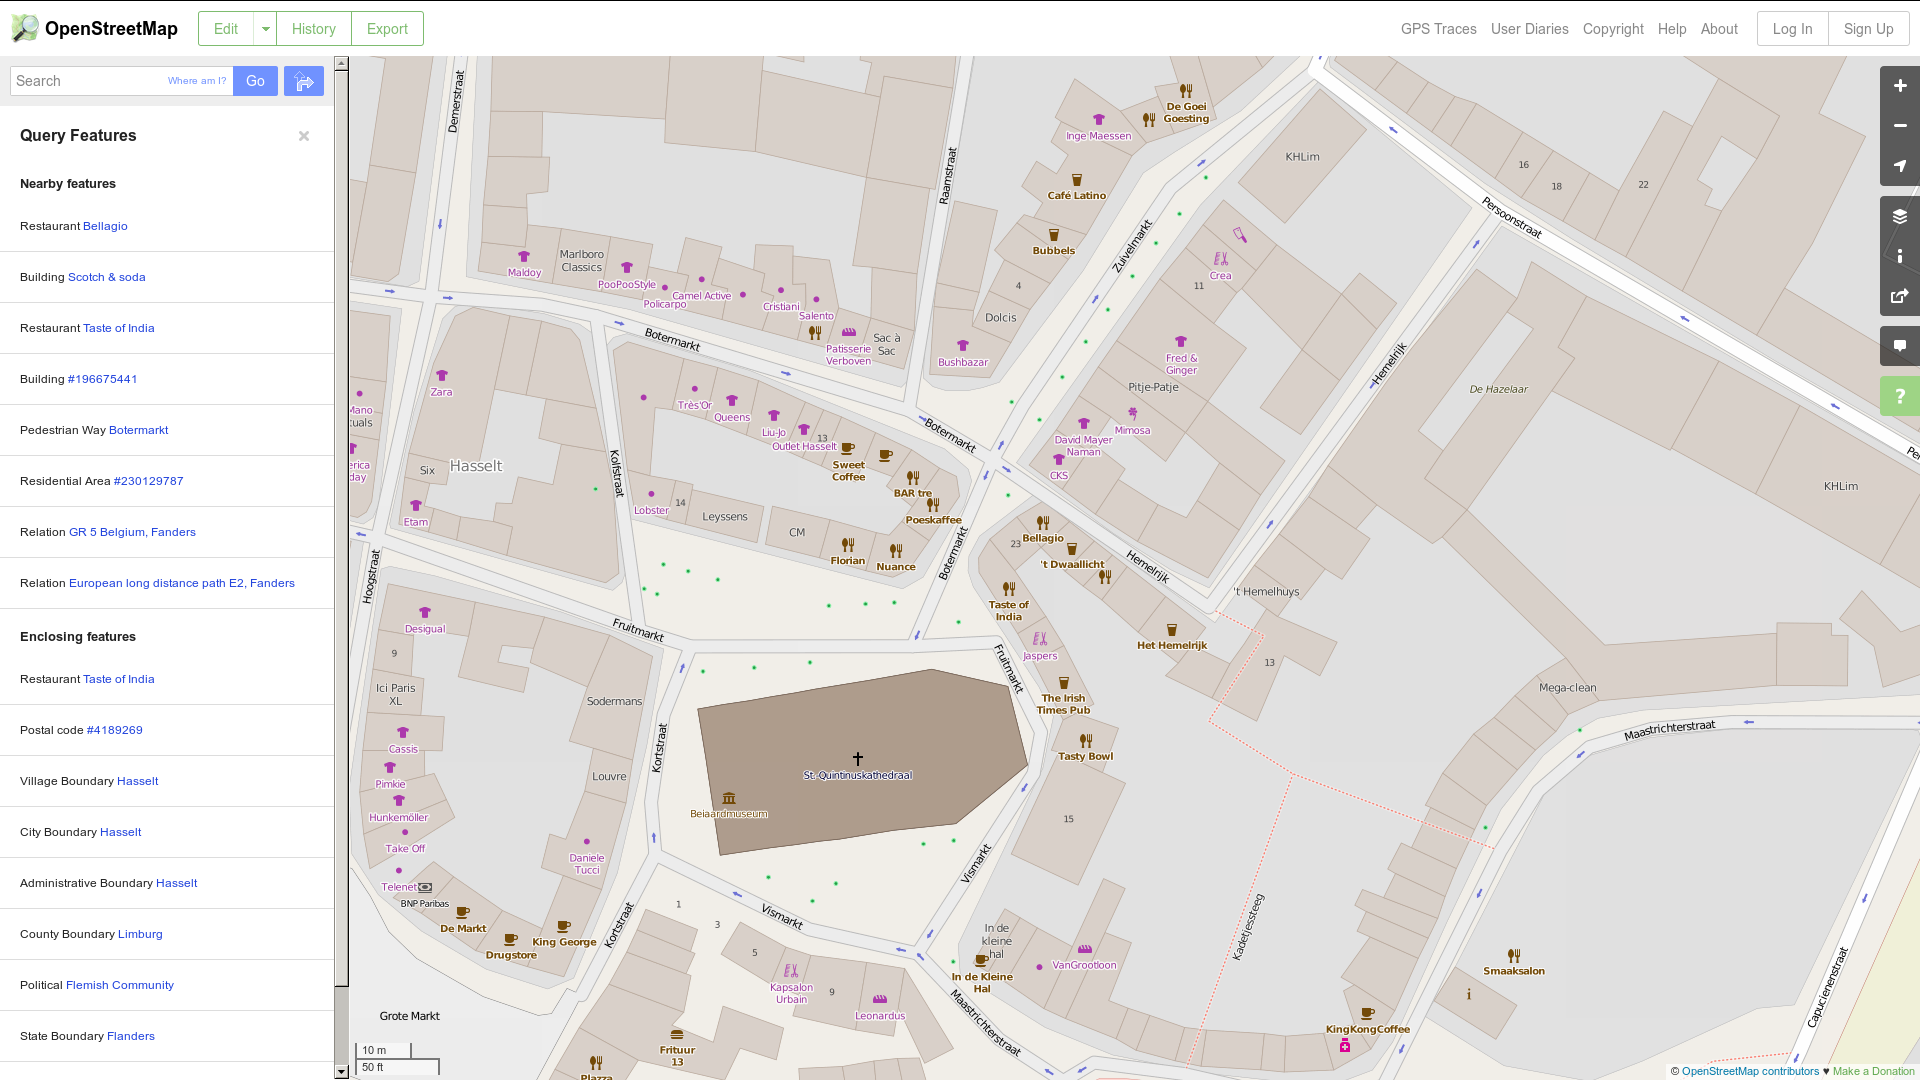
\includegraphics[width=\textwidth]{OSM_feature}}
\end{frame}

\begin{frame}
  \frametitle{Visualisierung}
  \Wider{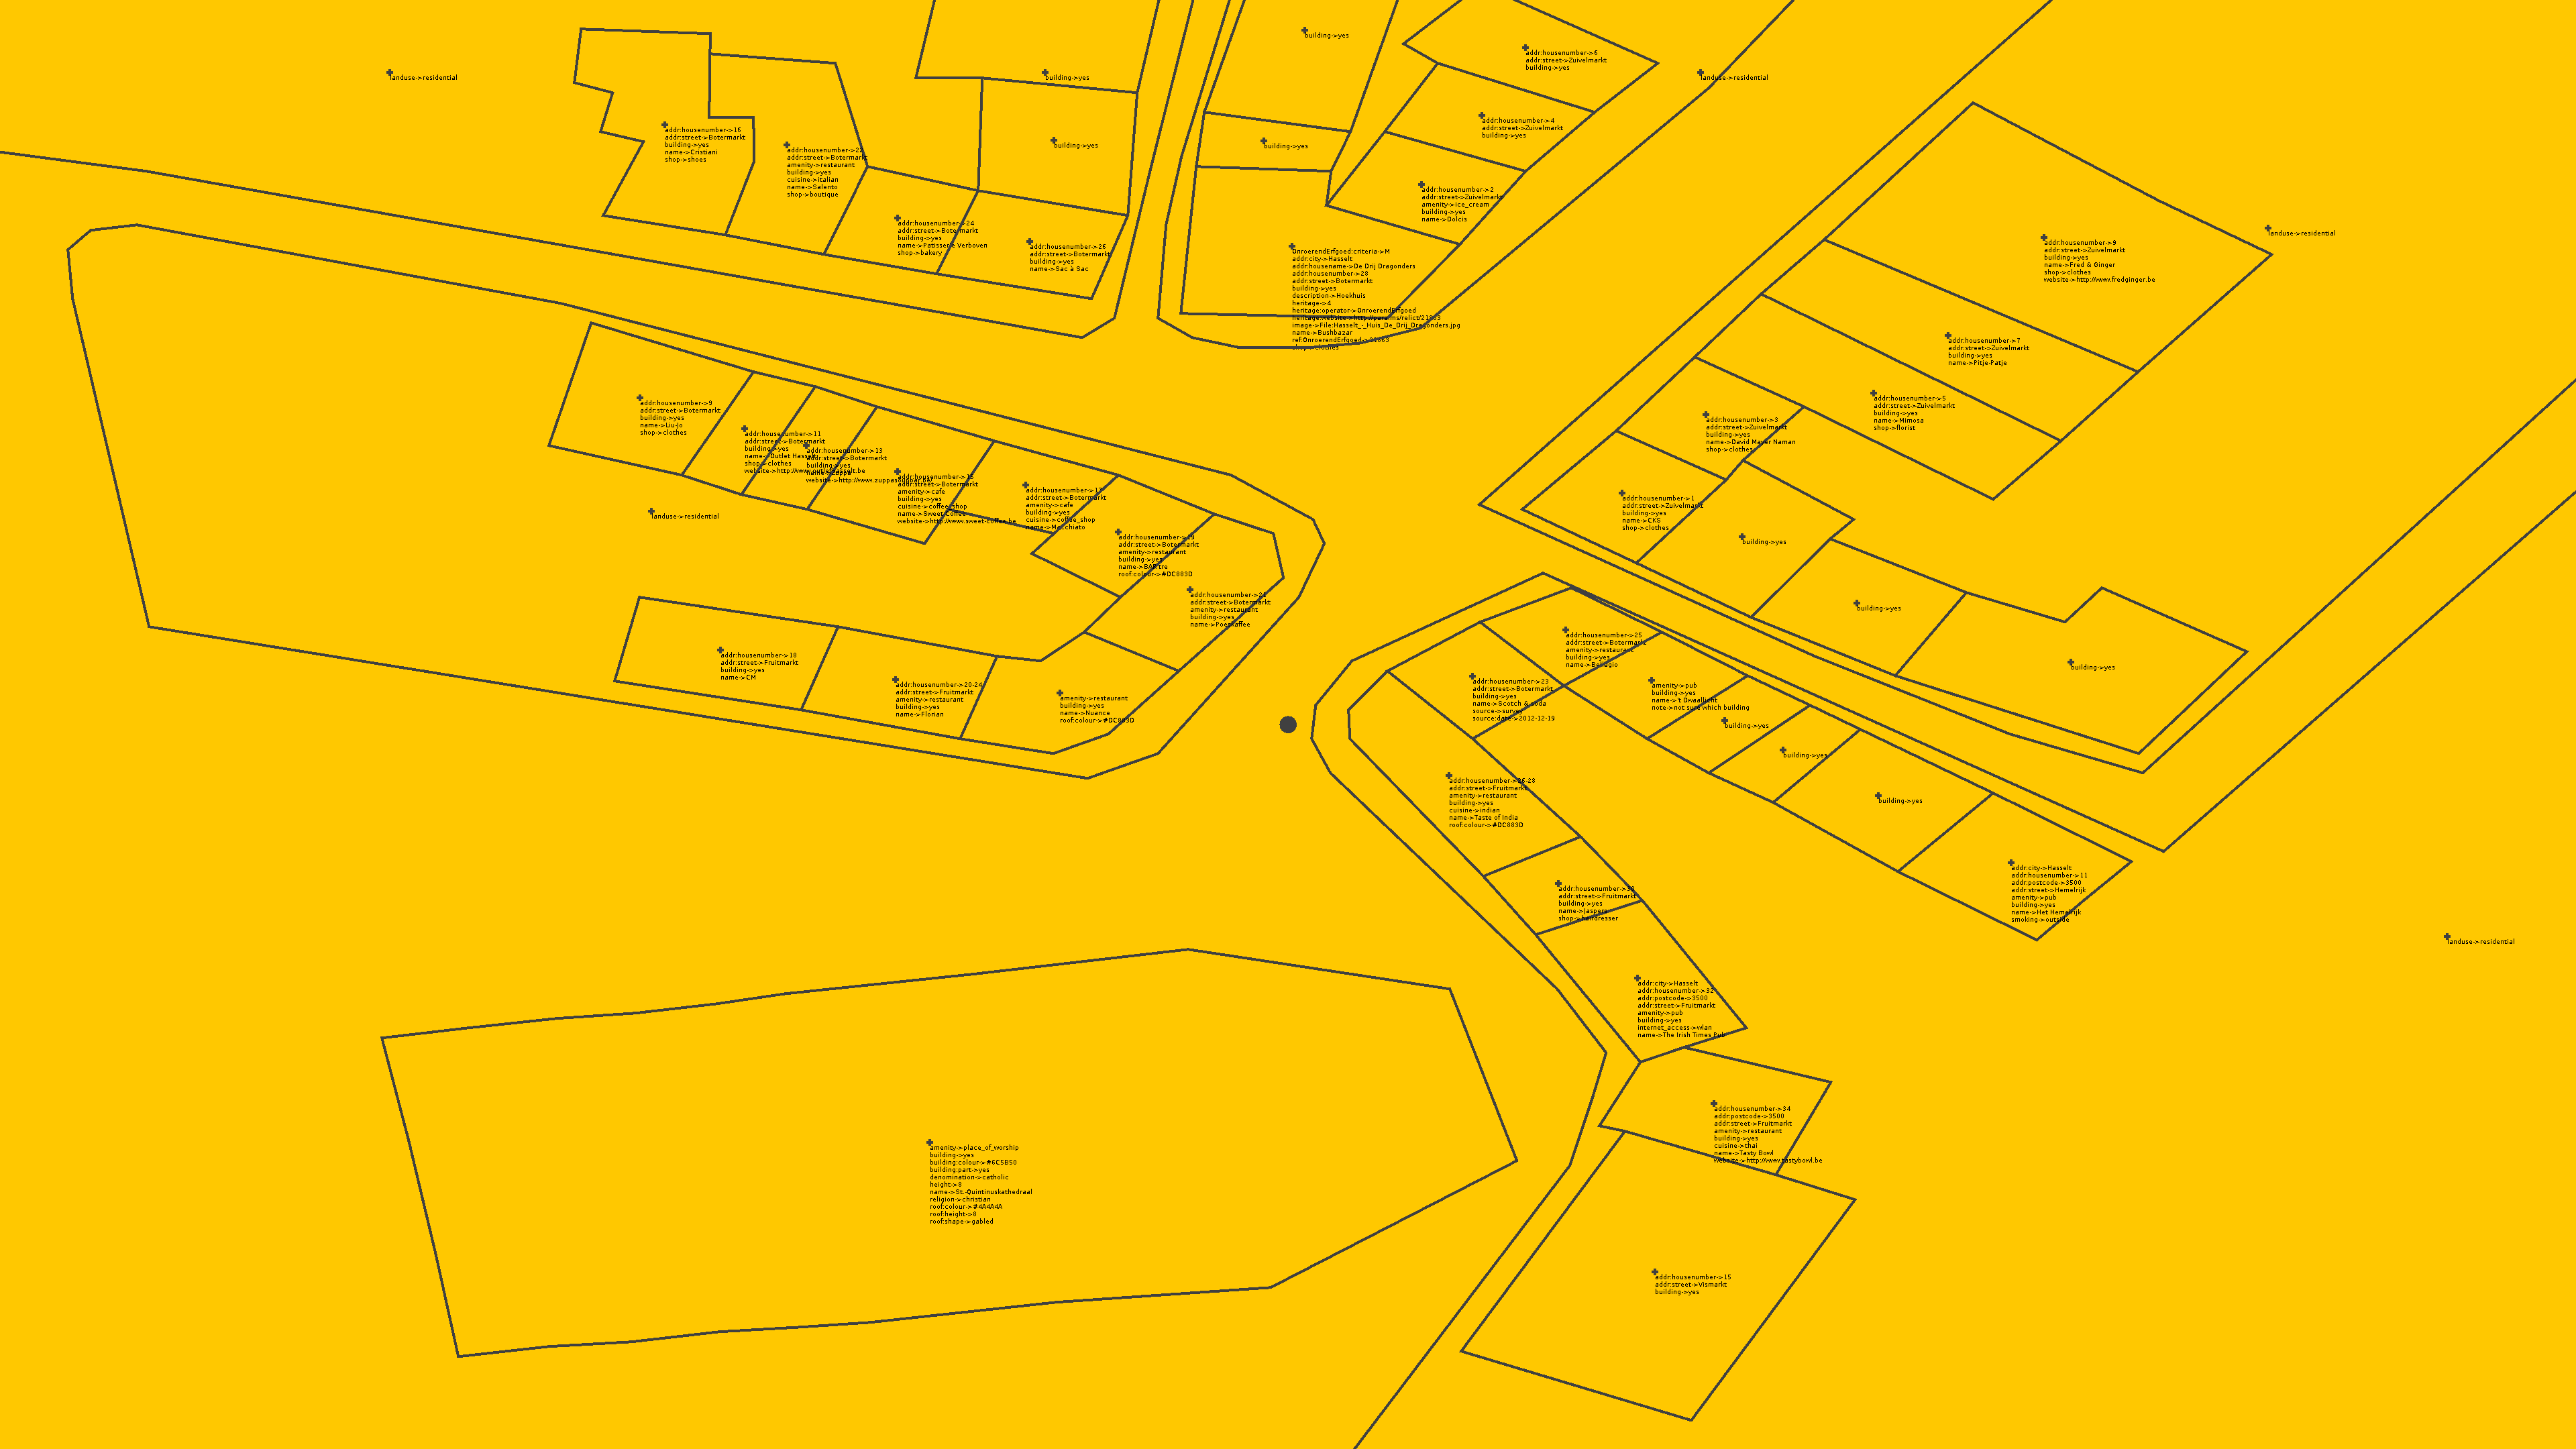
\includegraphics[width=\textwidth]{DataDrawer_raw}}
\end{frame}

\begin{frame}
  \frametitle{Visualisierung}
  \Wider{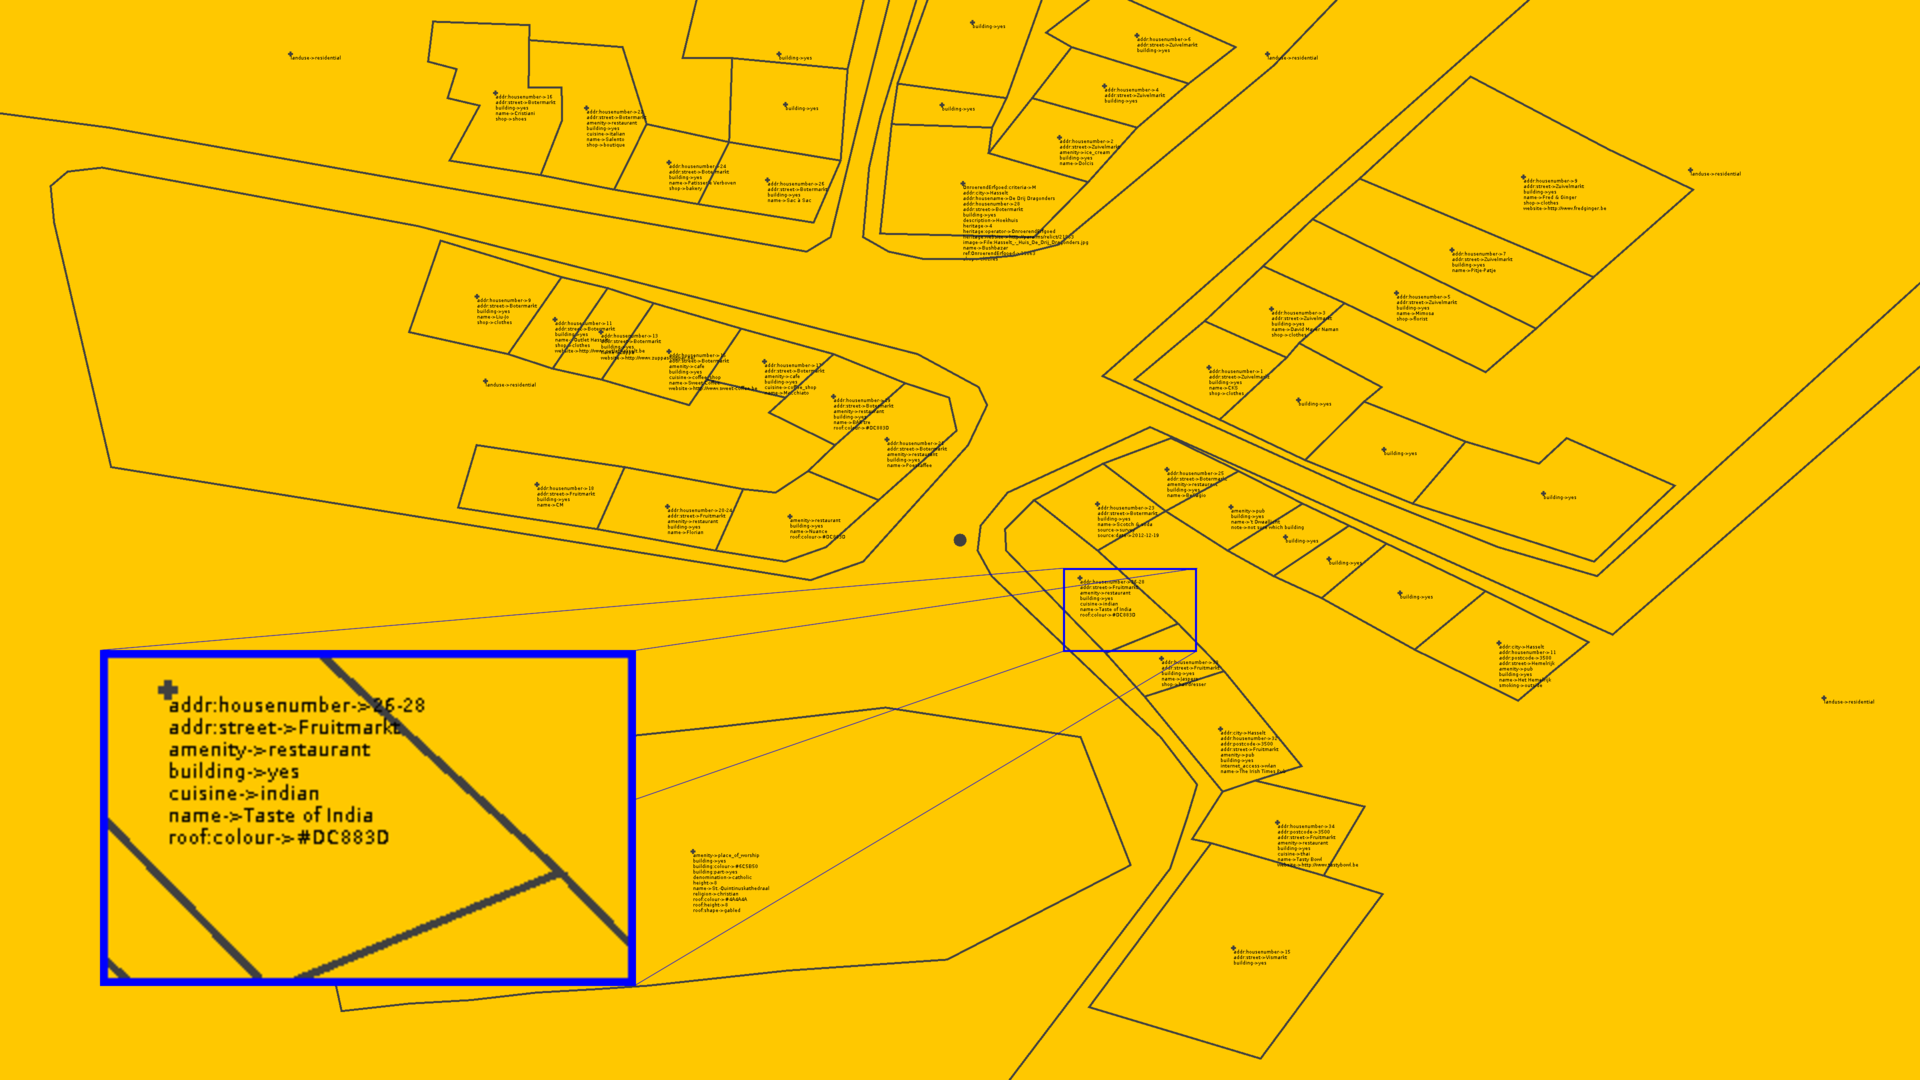
\includegraphics[width=\textwidth]{DataDrawer_raw_selected}}
\end{frame}

\begin{frame}
  \frametitle{Visualisierung}
  \Wider{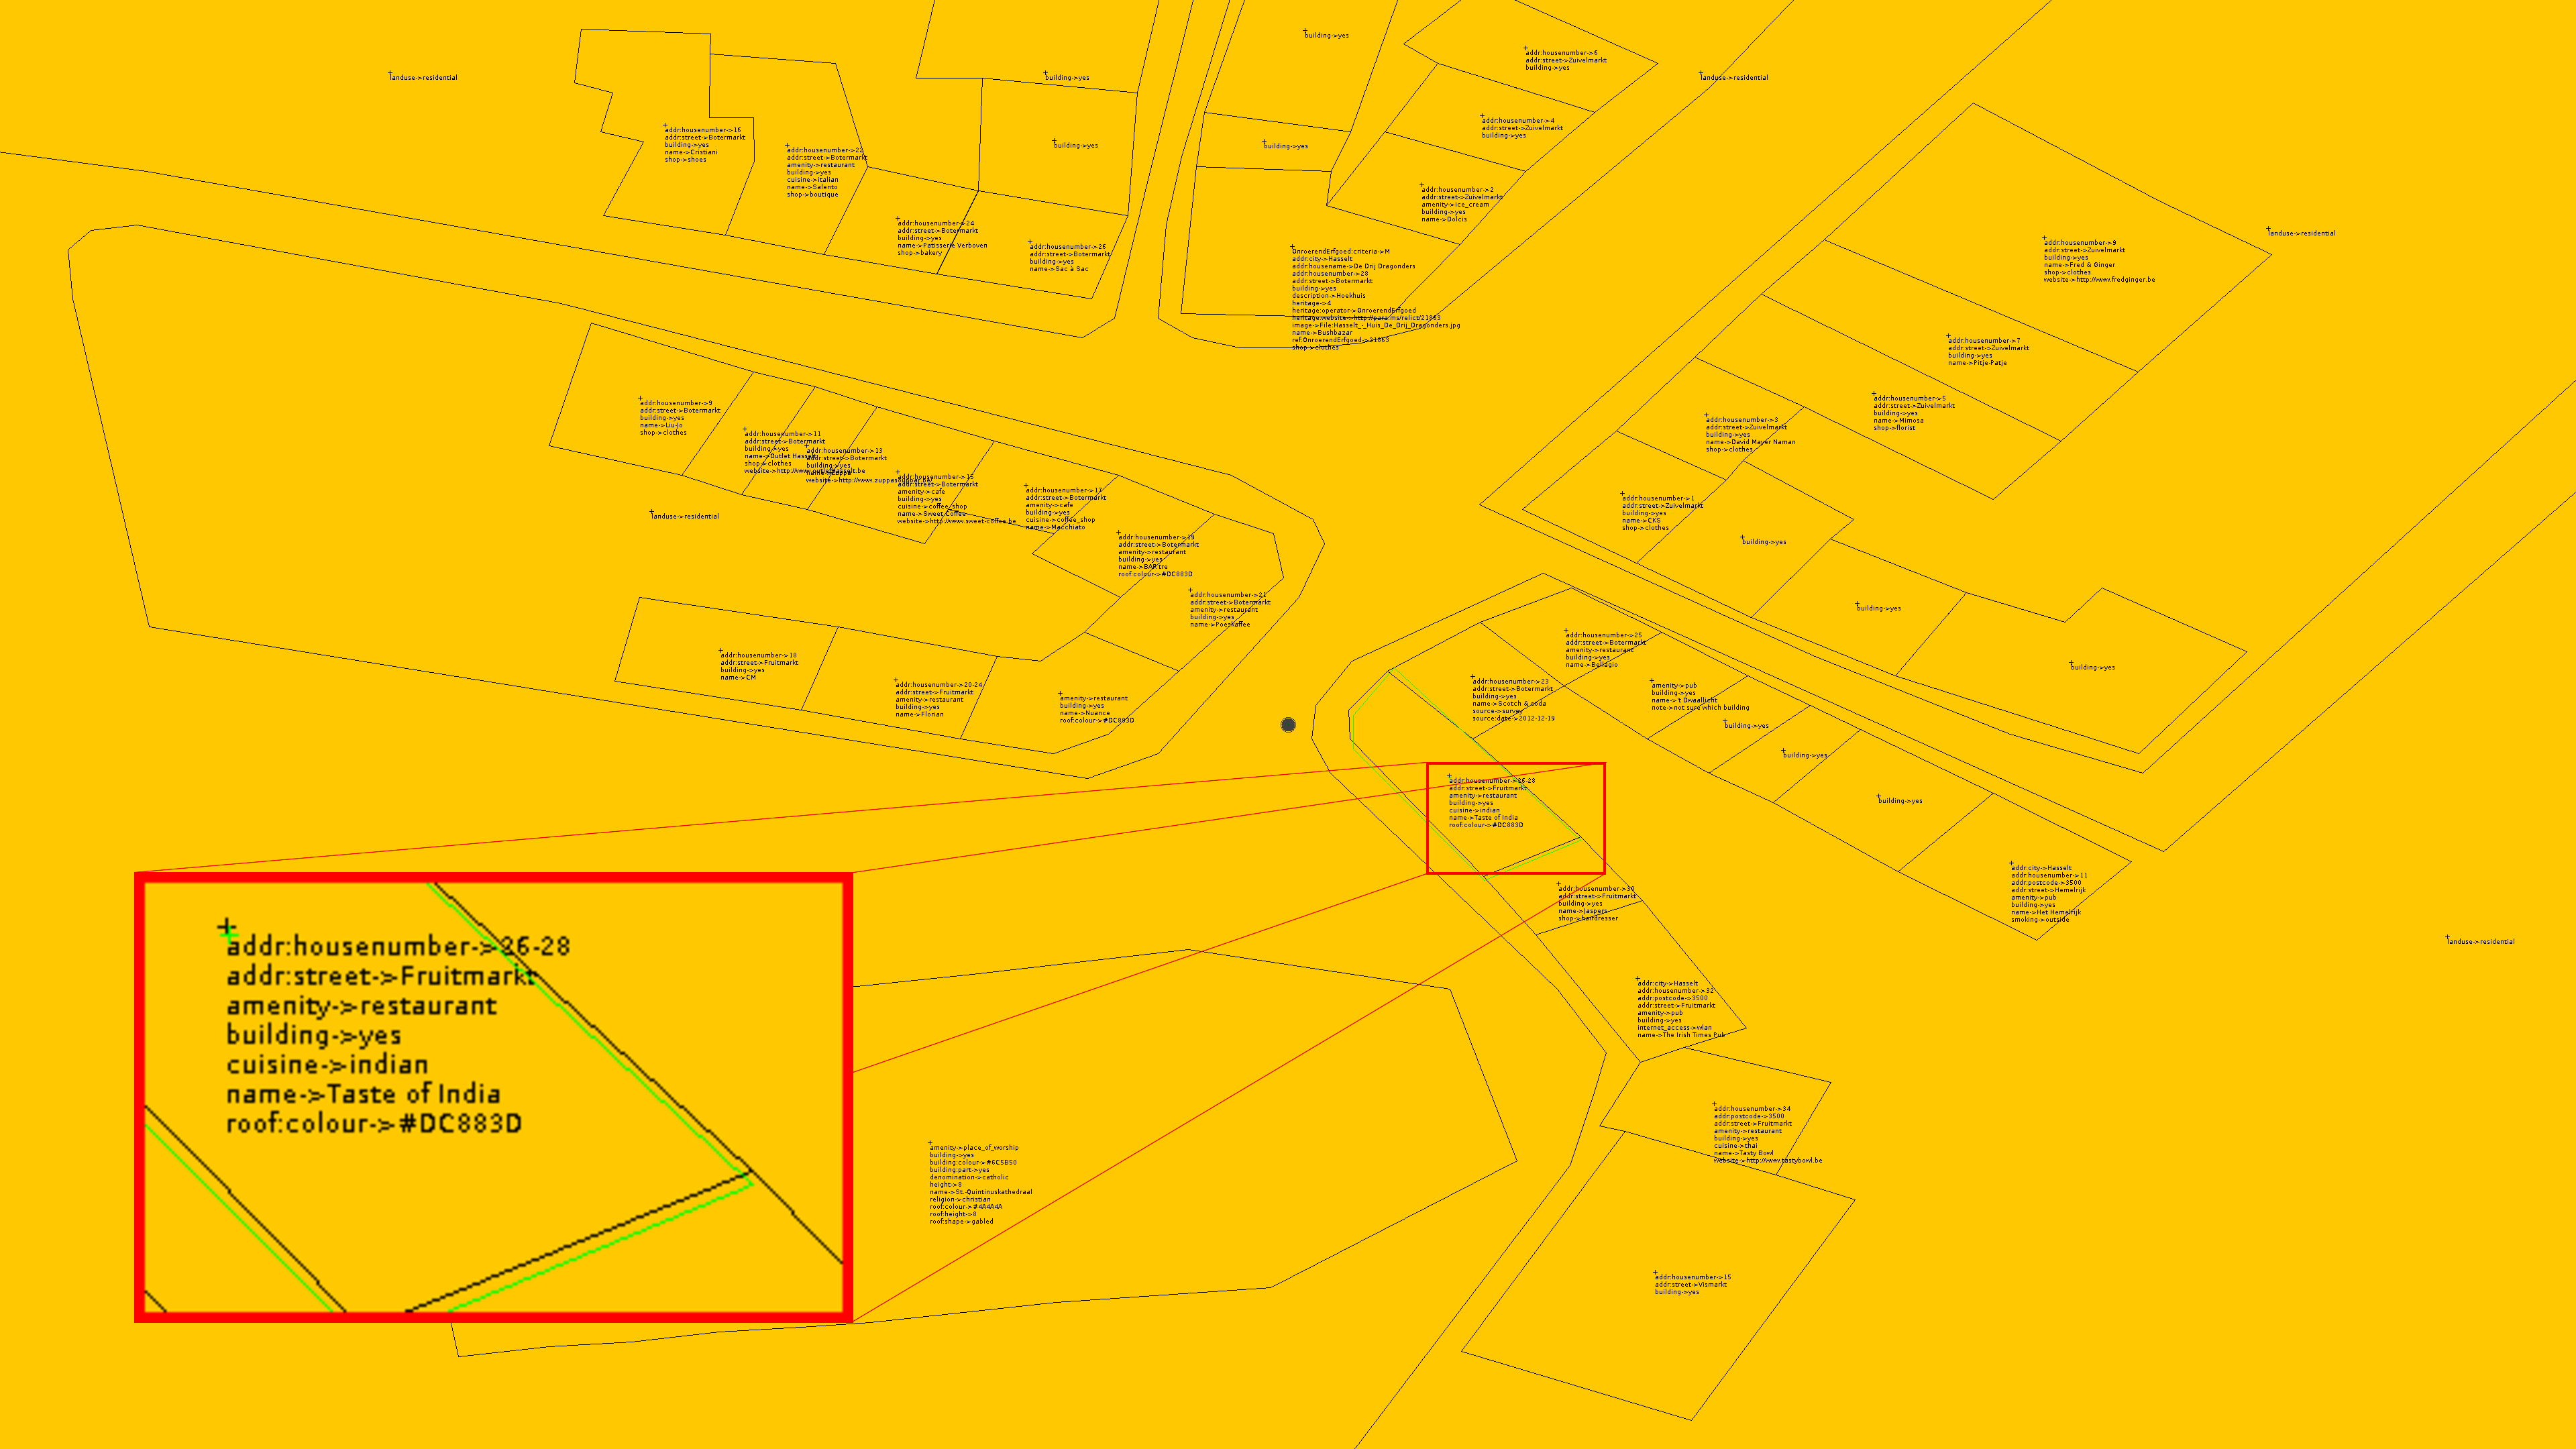
\includegraphics[width=\textwidth]{DataDrawer_truth_selected}}
\end{frame}

\begin{frame}
  \frametitle{Visualisierung}
  \Wider{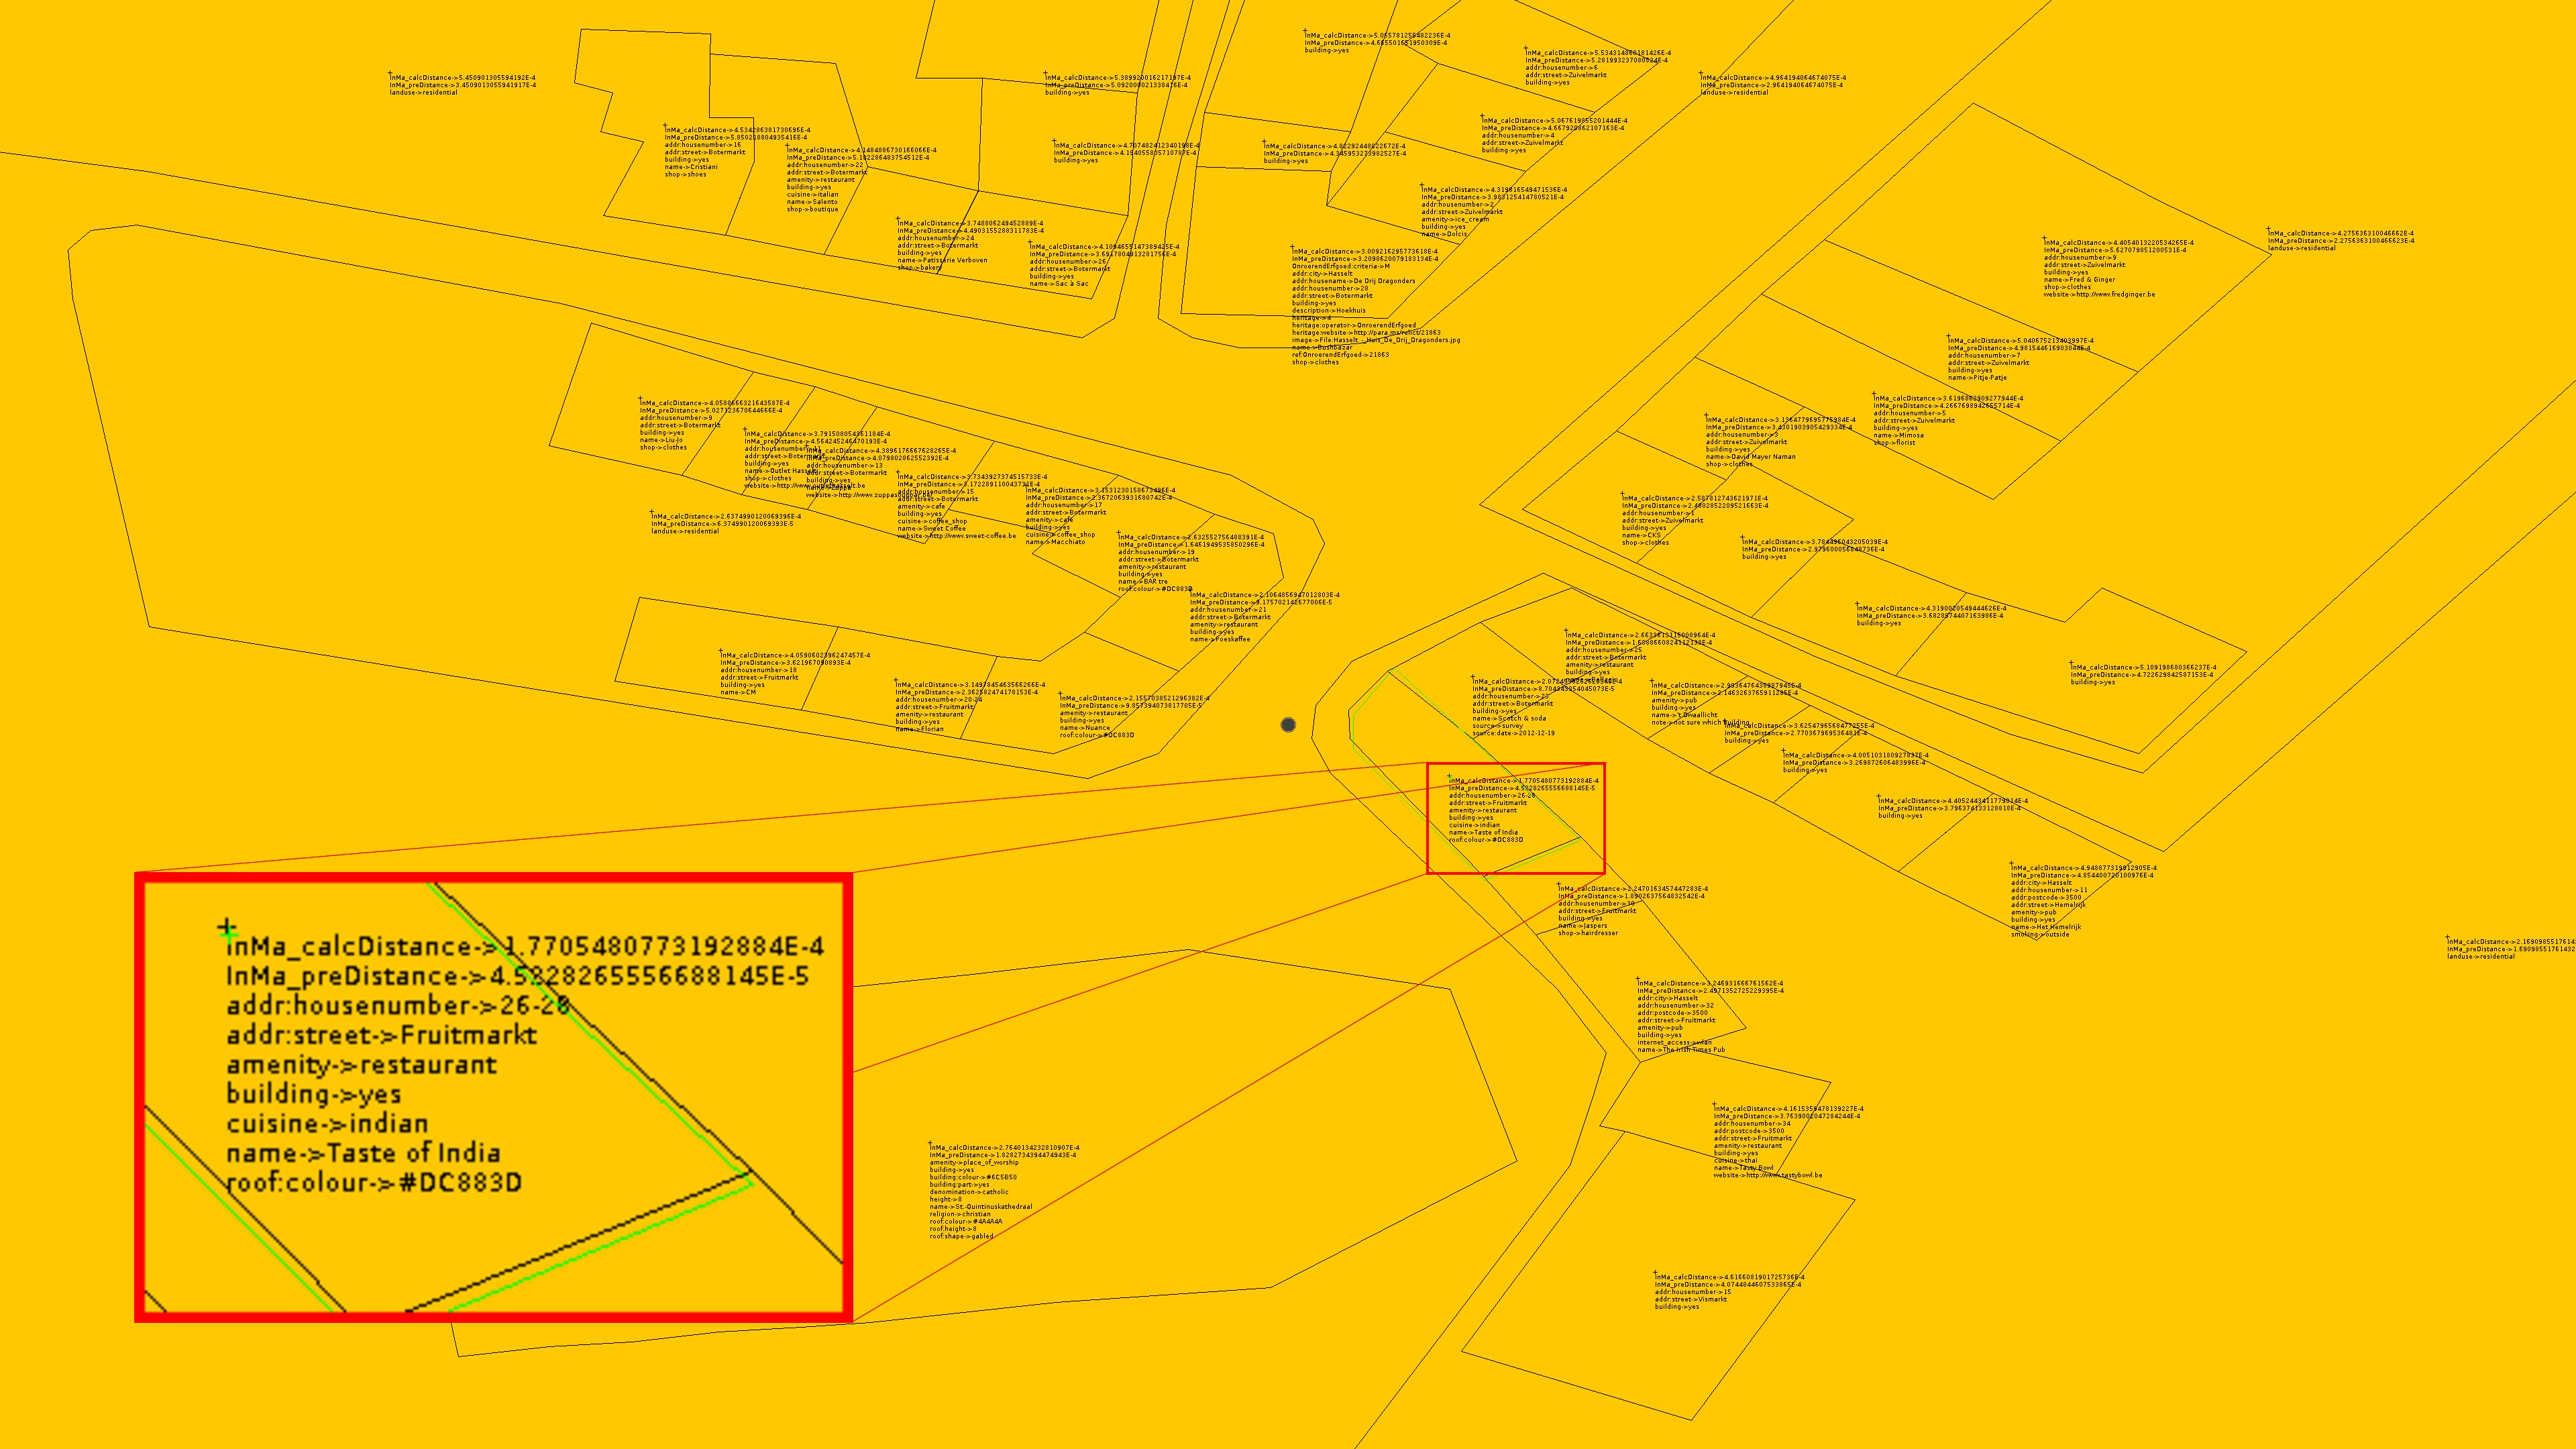
\includegraphics[width=\textwidth]{DataDrawer_dist_selected}}
\end{frame}

\begin{frame}
  \frametitle{Visualisierung}
  \Wider{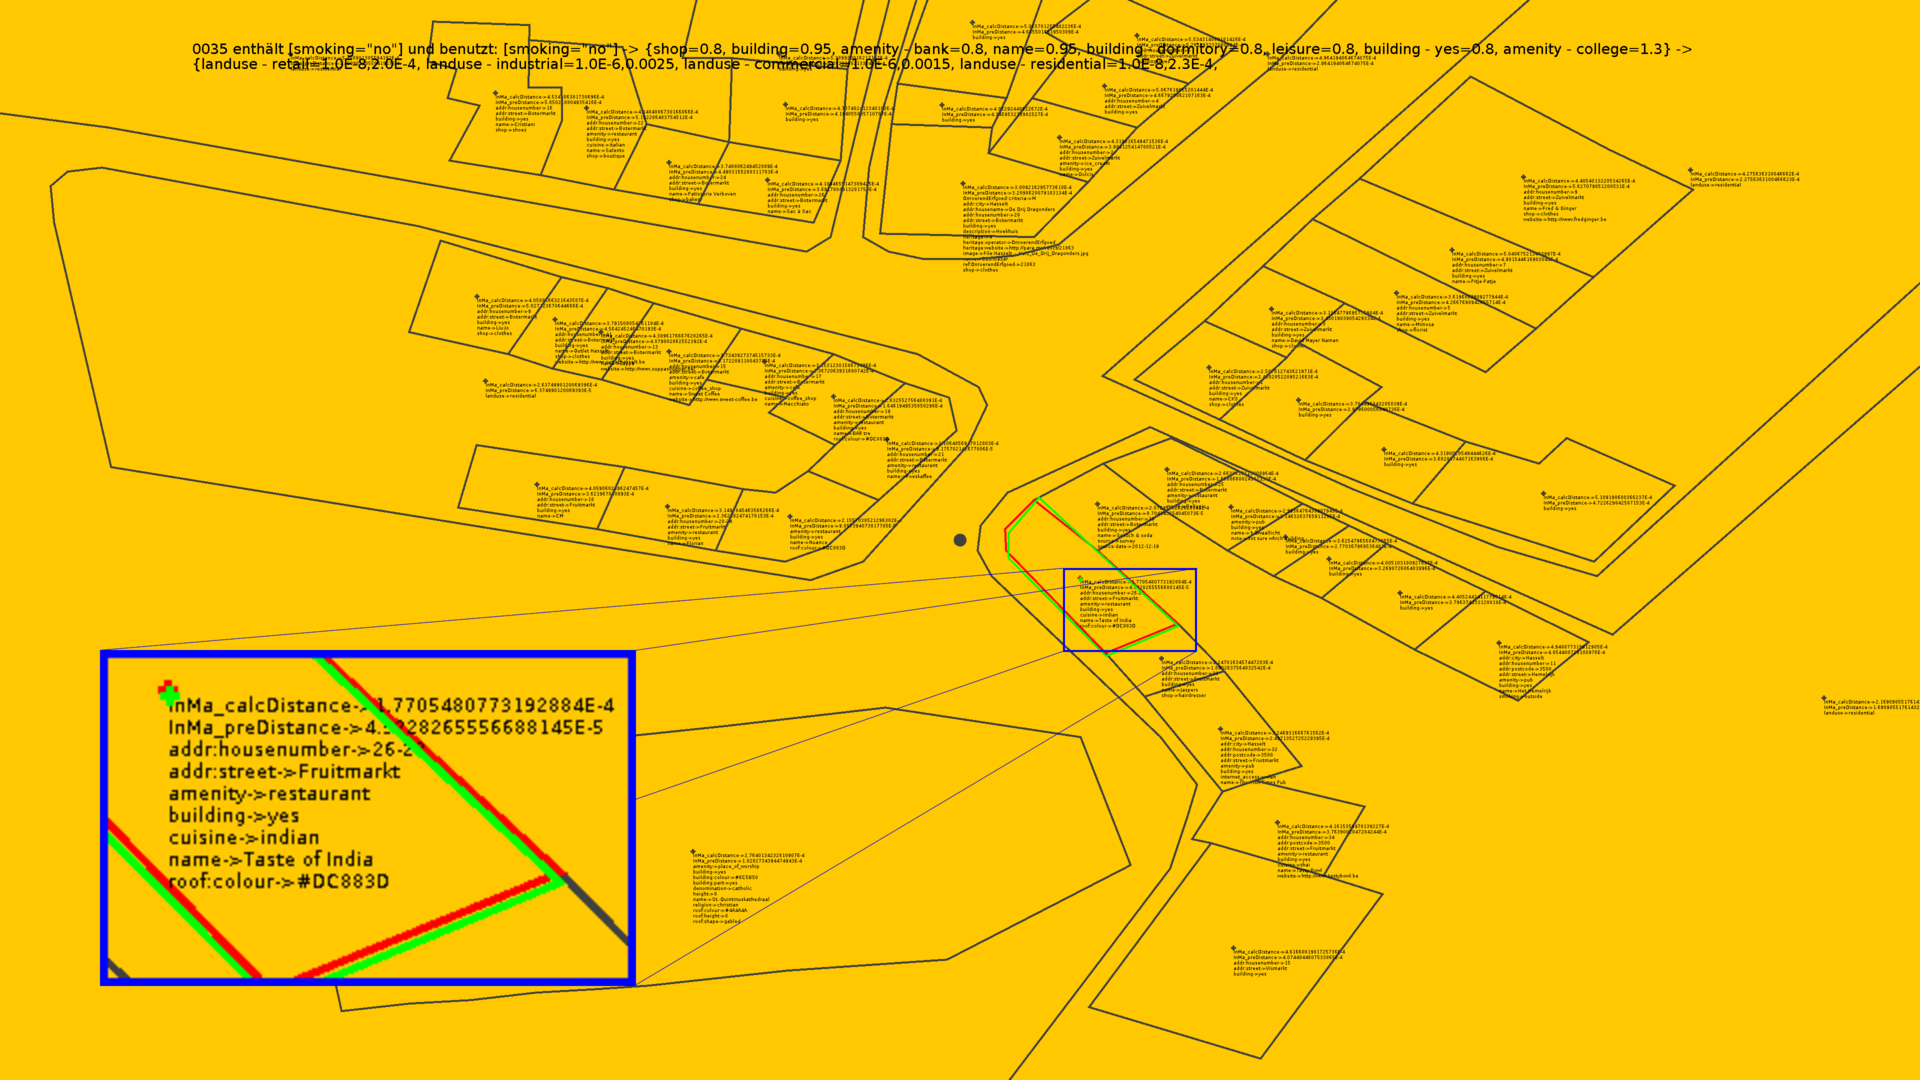
\includegraphics[width=\textwidth]{DataDrawer_rules_selected}}
\end{frame}

\begin{frame}
  \frametitle{Visualisierung}
  \Wider{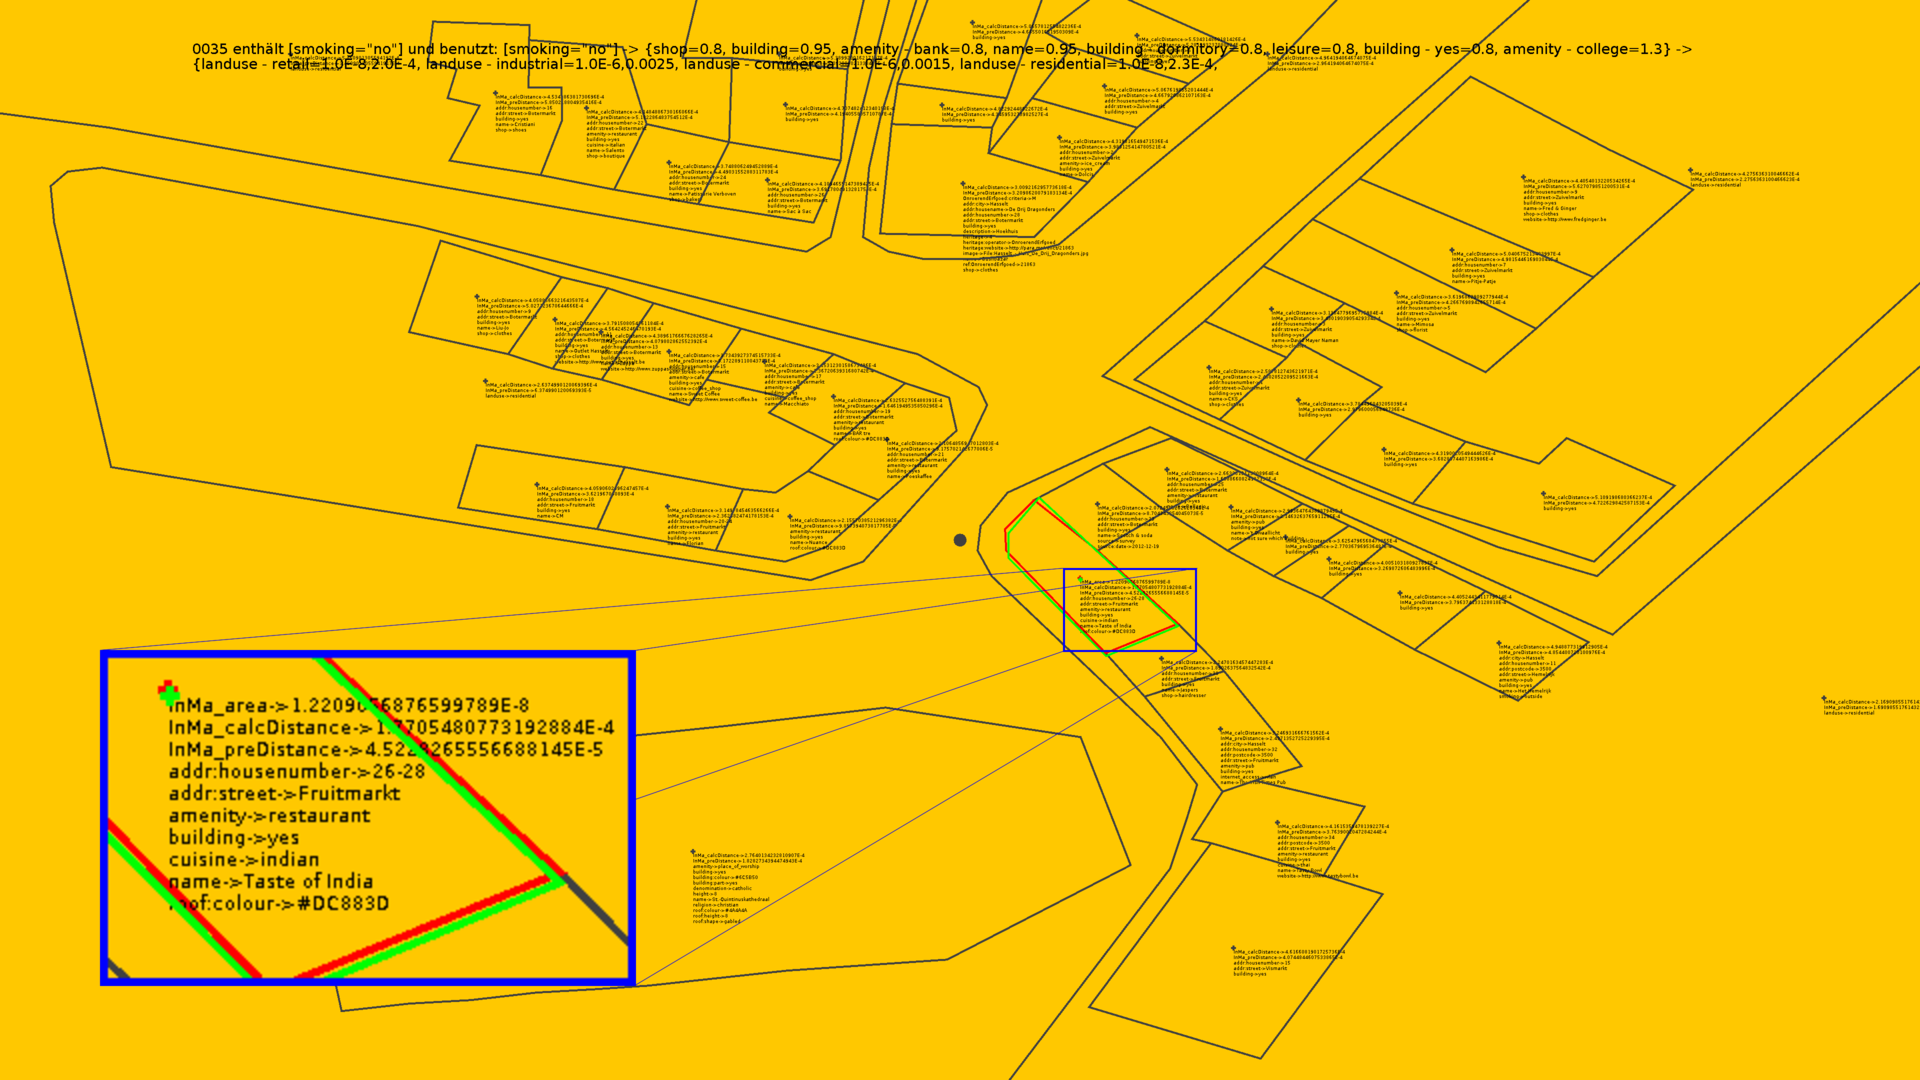
\includegraphics[width=\textwidth]{DataDrawer_area_selected}}
\end{frame}

\begin{frame}
  \frametitle{Coverage}
  \begin{equation*}
    Coverage = \frac{Area_{intersection}}{max(Area_{guesspolygon},Area_{loesungspolygon})}
  \end{equation*}
\\
  \begin{equation*}
    Coverage \in {0..1}
  \end{equation*}
%%%%%%%%%%%%%%%%%%%%%%%%%%%%%%%%%%%%%%%%%%%%%%%%%%%%%%%%%%%%%%%%%%%%%%%%%%%%%%%%
% Vielleicht hier 3 kleine Beispiele für Coverage.
% 0: intersection = null
% 1: intersection = lösung  % oder beliebige andere
% 0.1: Lösung ist 1/10 von guess groß und liegt in ihr drinne
%%%%%%%%%%%%%%%%%%%%%%%%%%%%%%%%%%%%%%%%%%%%%%%%%%%%%%%%%%%%%%%%%%%%%%%%%%%%%%%%
\end{frame}

\begin{frame}
  \frametitle{Naiver Ansatz}
  \begin{center}
  \huge{Coverage = 49,6 \%}
  \end{center}
\end{frame}

\begin{frame}
  \frametitle{Gewichteter Ansatz}
  \begin{center}
  \huge{Coverage = 69,8 \%}
  \end{center}
  \begin{center}
  Naive Coverage = 49,6 \%
  \end{center}
\end{frame}


\begin{frame}
  \frametitle{Unvollständige Datensätze \hfill Nr. 38}
  \Wider{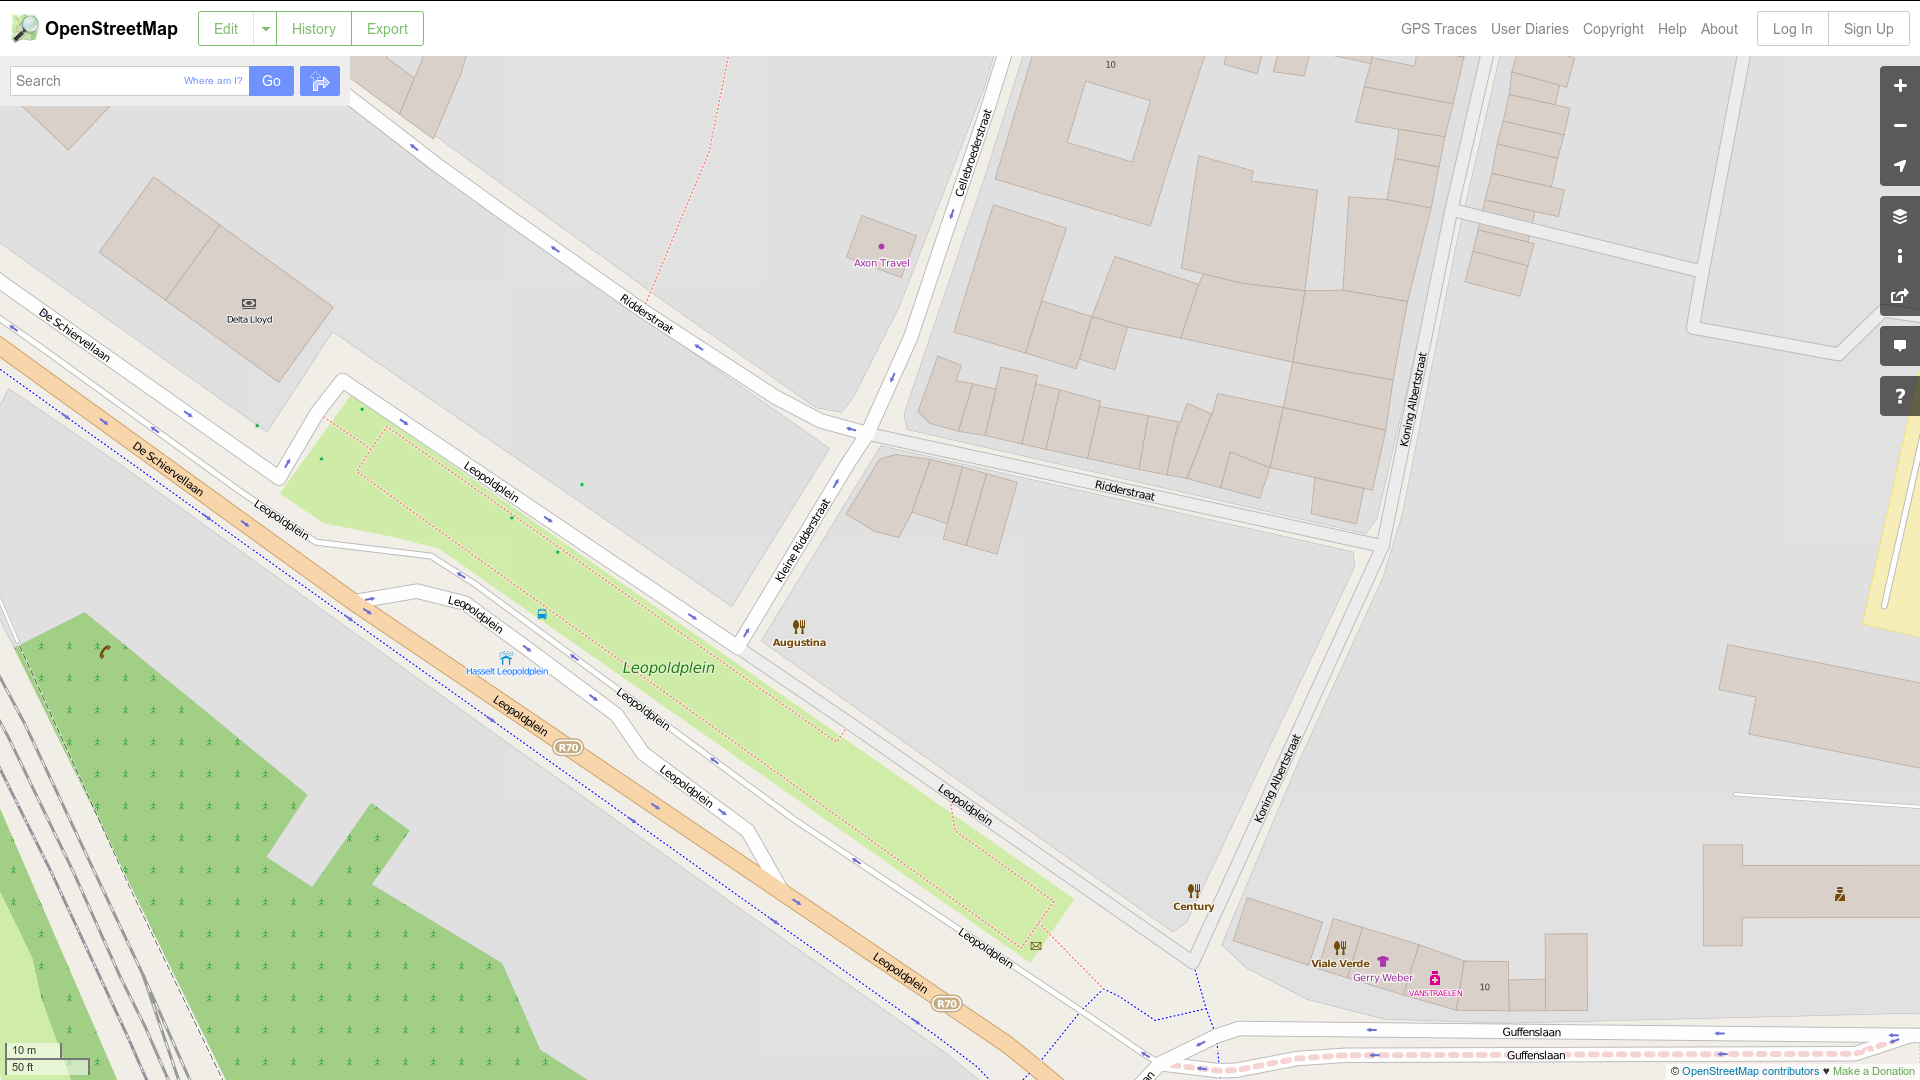
\includegraphics[width=\textwidth]{unvollstaendig}}
\end{frame}


\begin{frame}
  \frametitle{Unvollständige Datensätze \hfill Nr. 38}
  \Wider{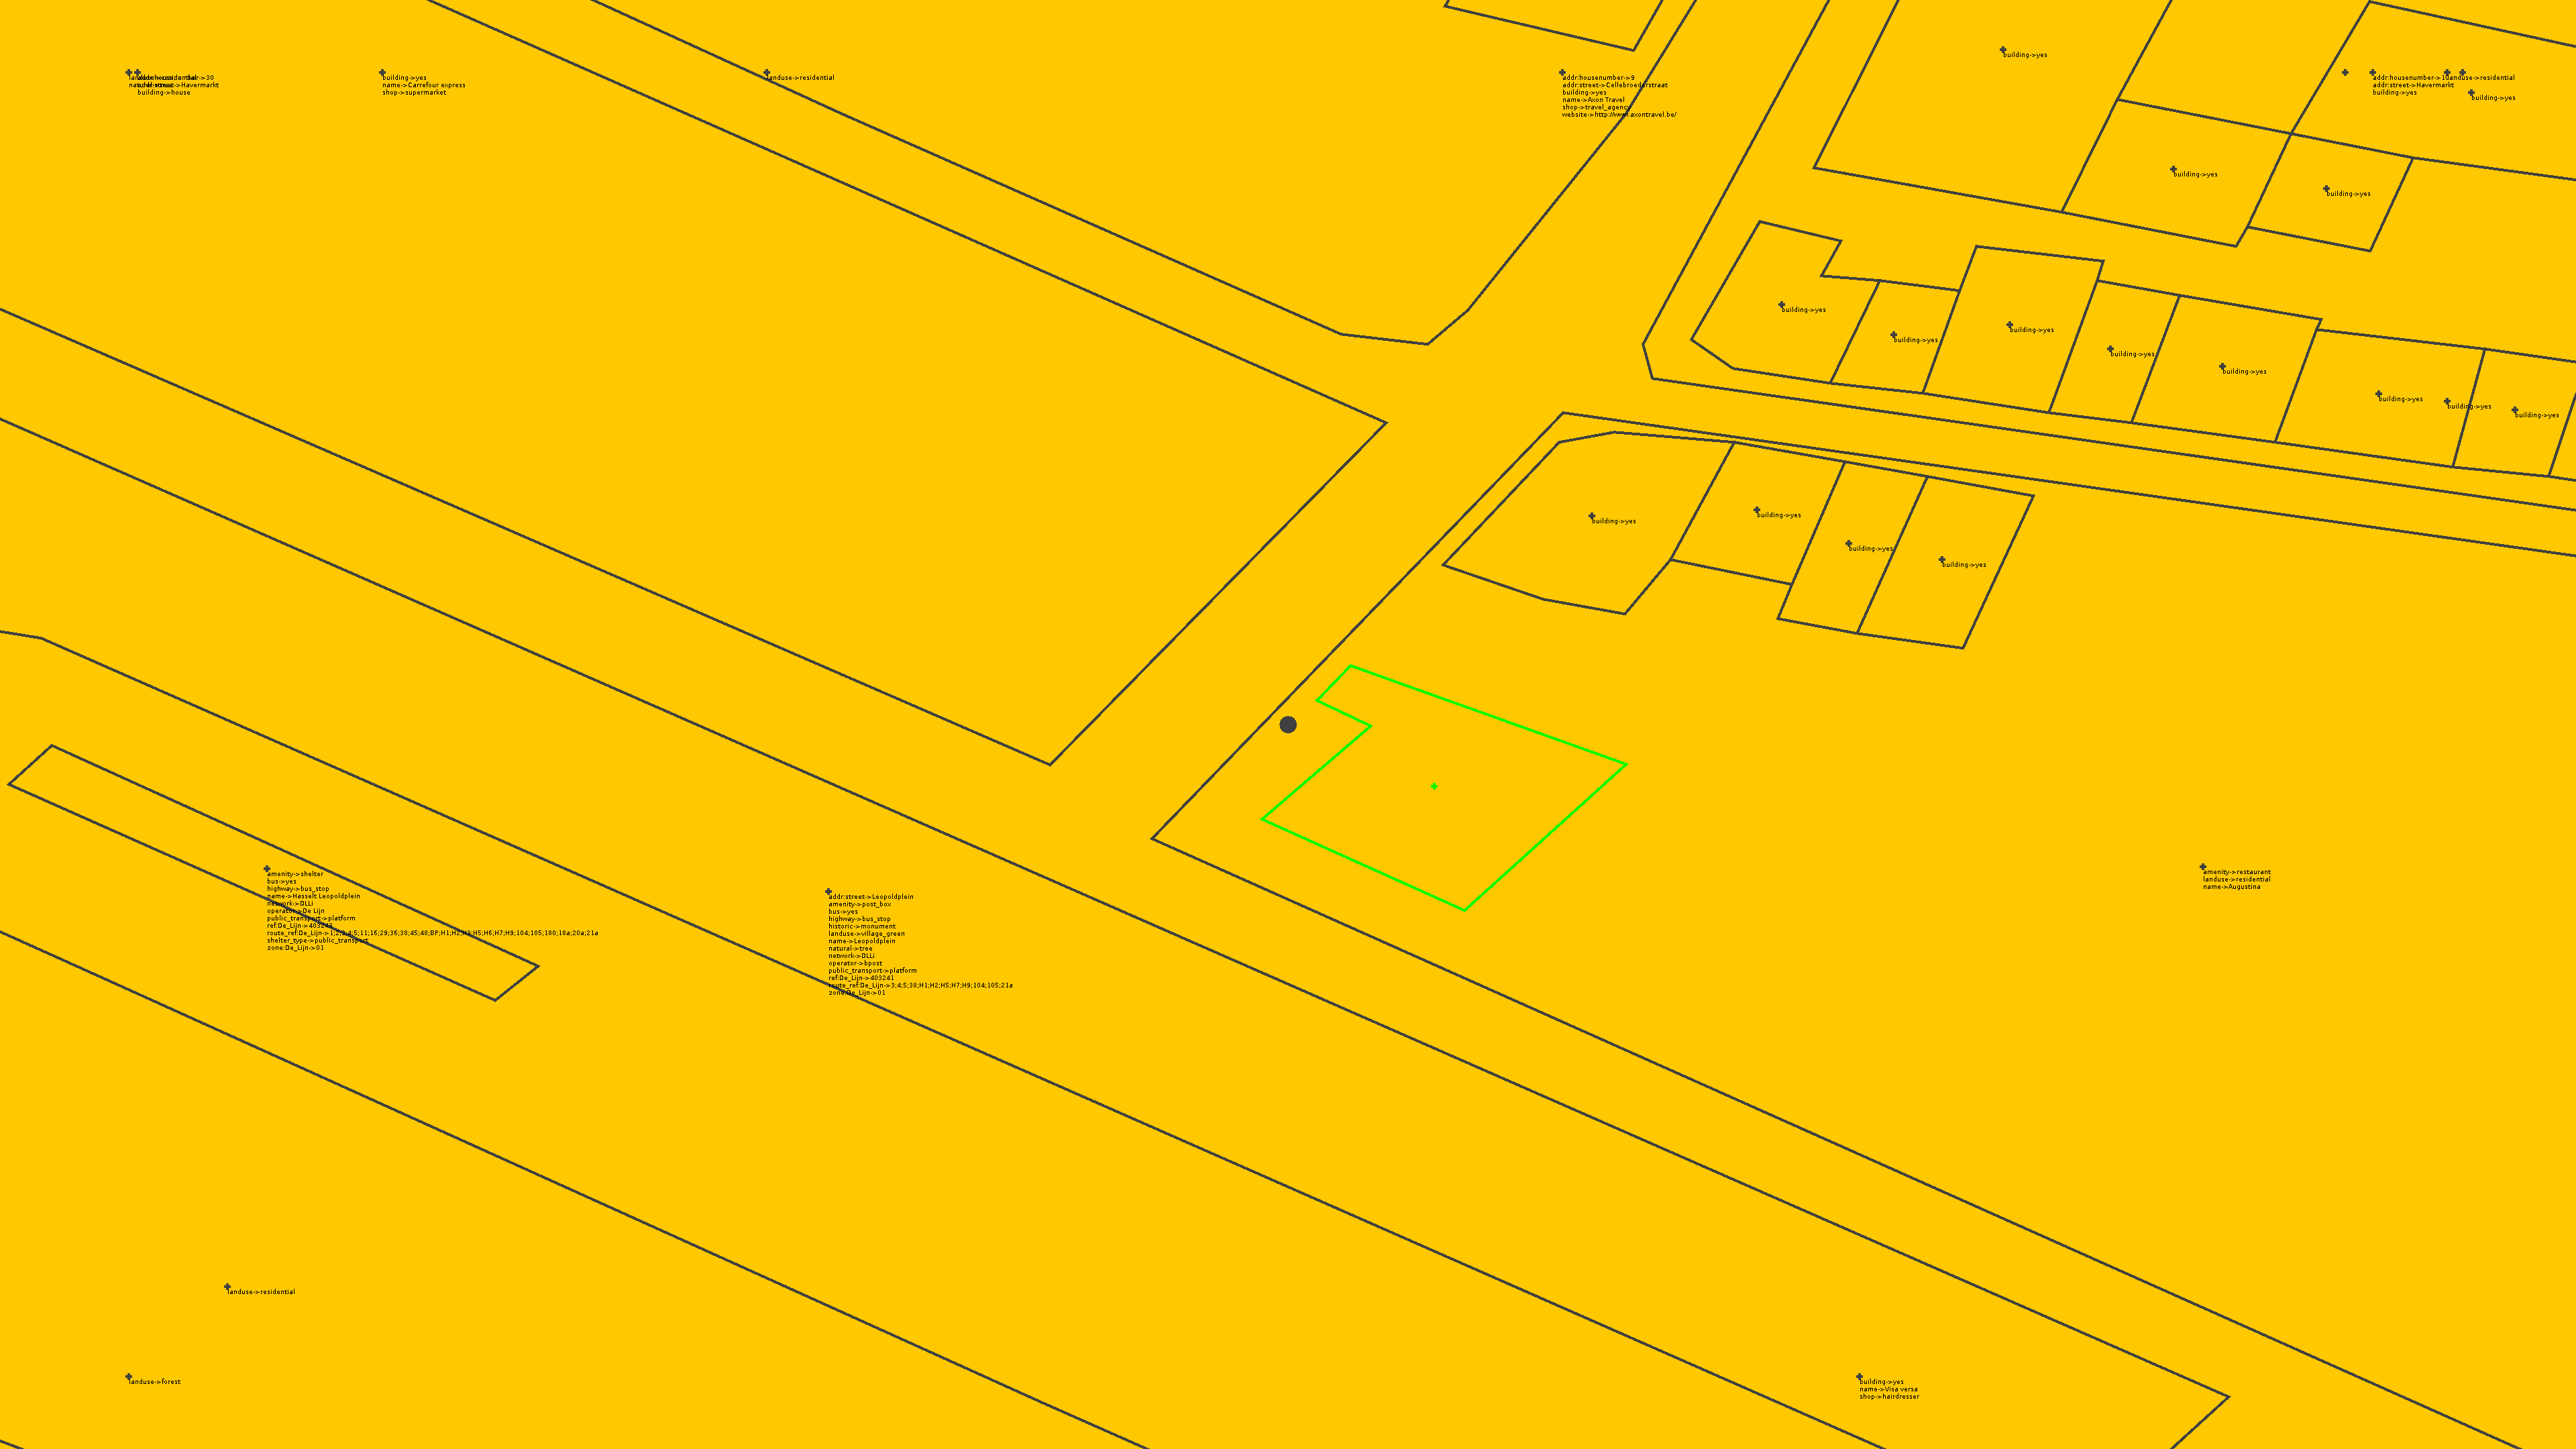
\includegraphics[width=\textwidth]{unvoll_ours}}
\end{frame}


\begin{frame}
  \frametitle{Unvollständige Datensätze \hfill Nr. 38}
  \Wider{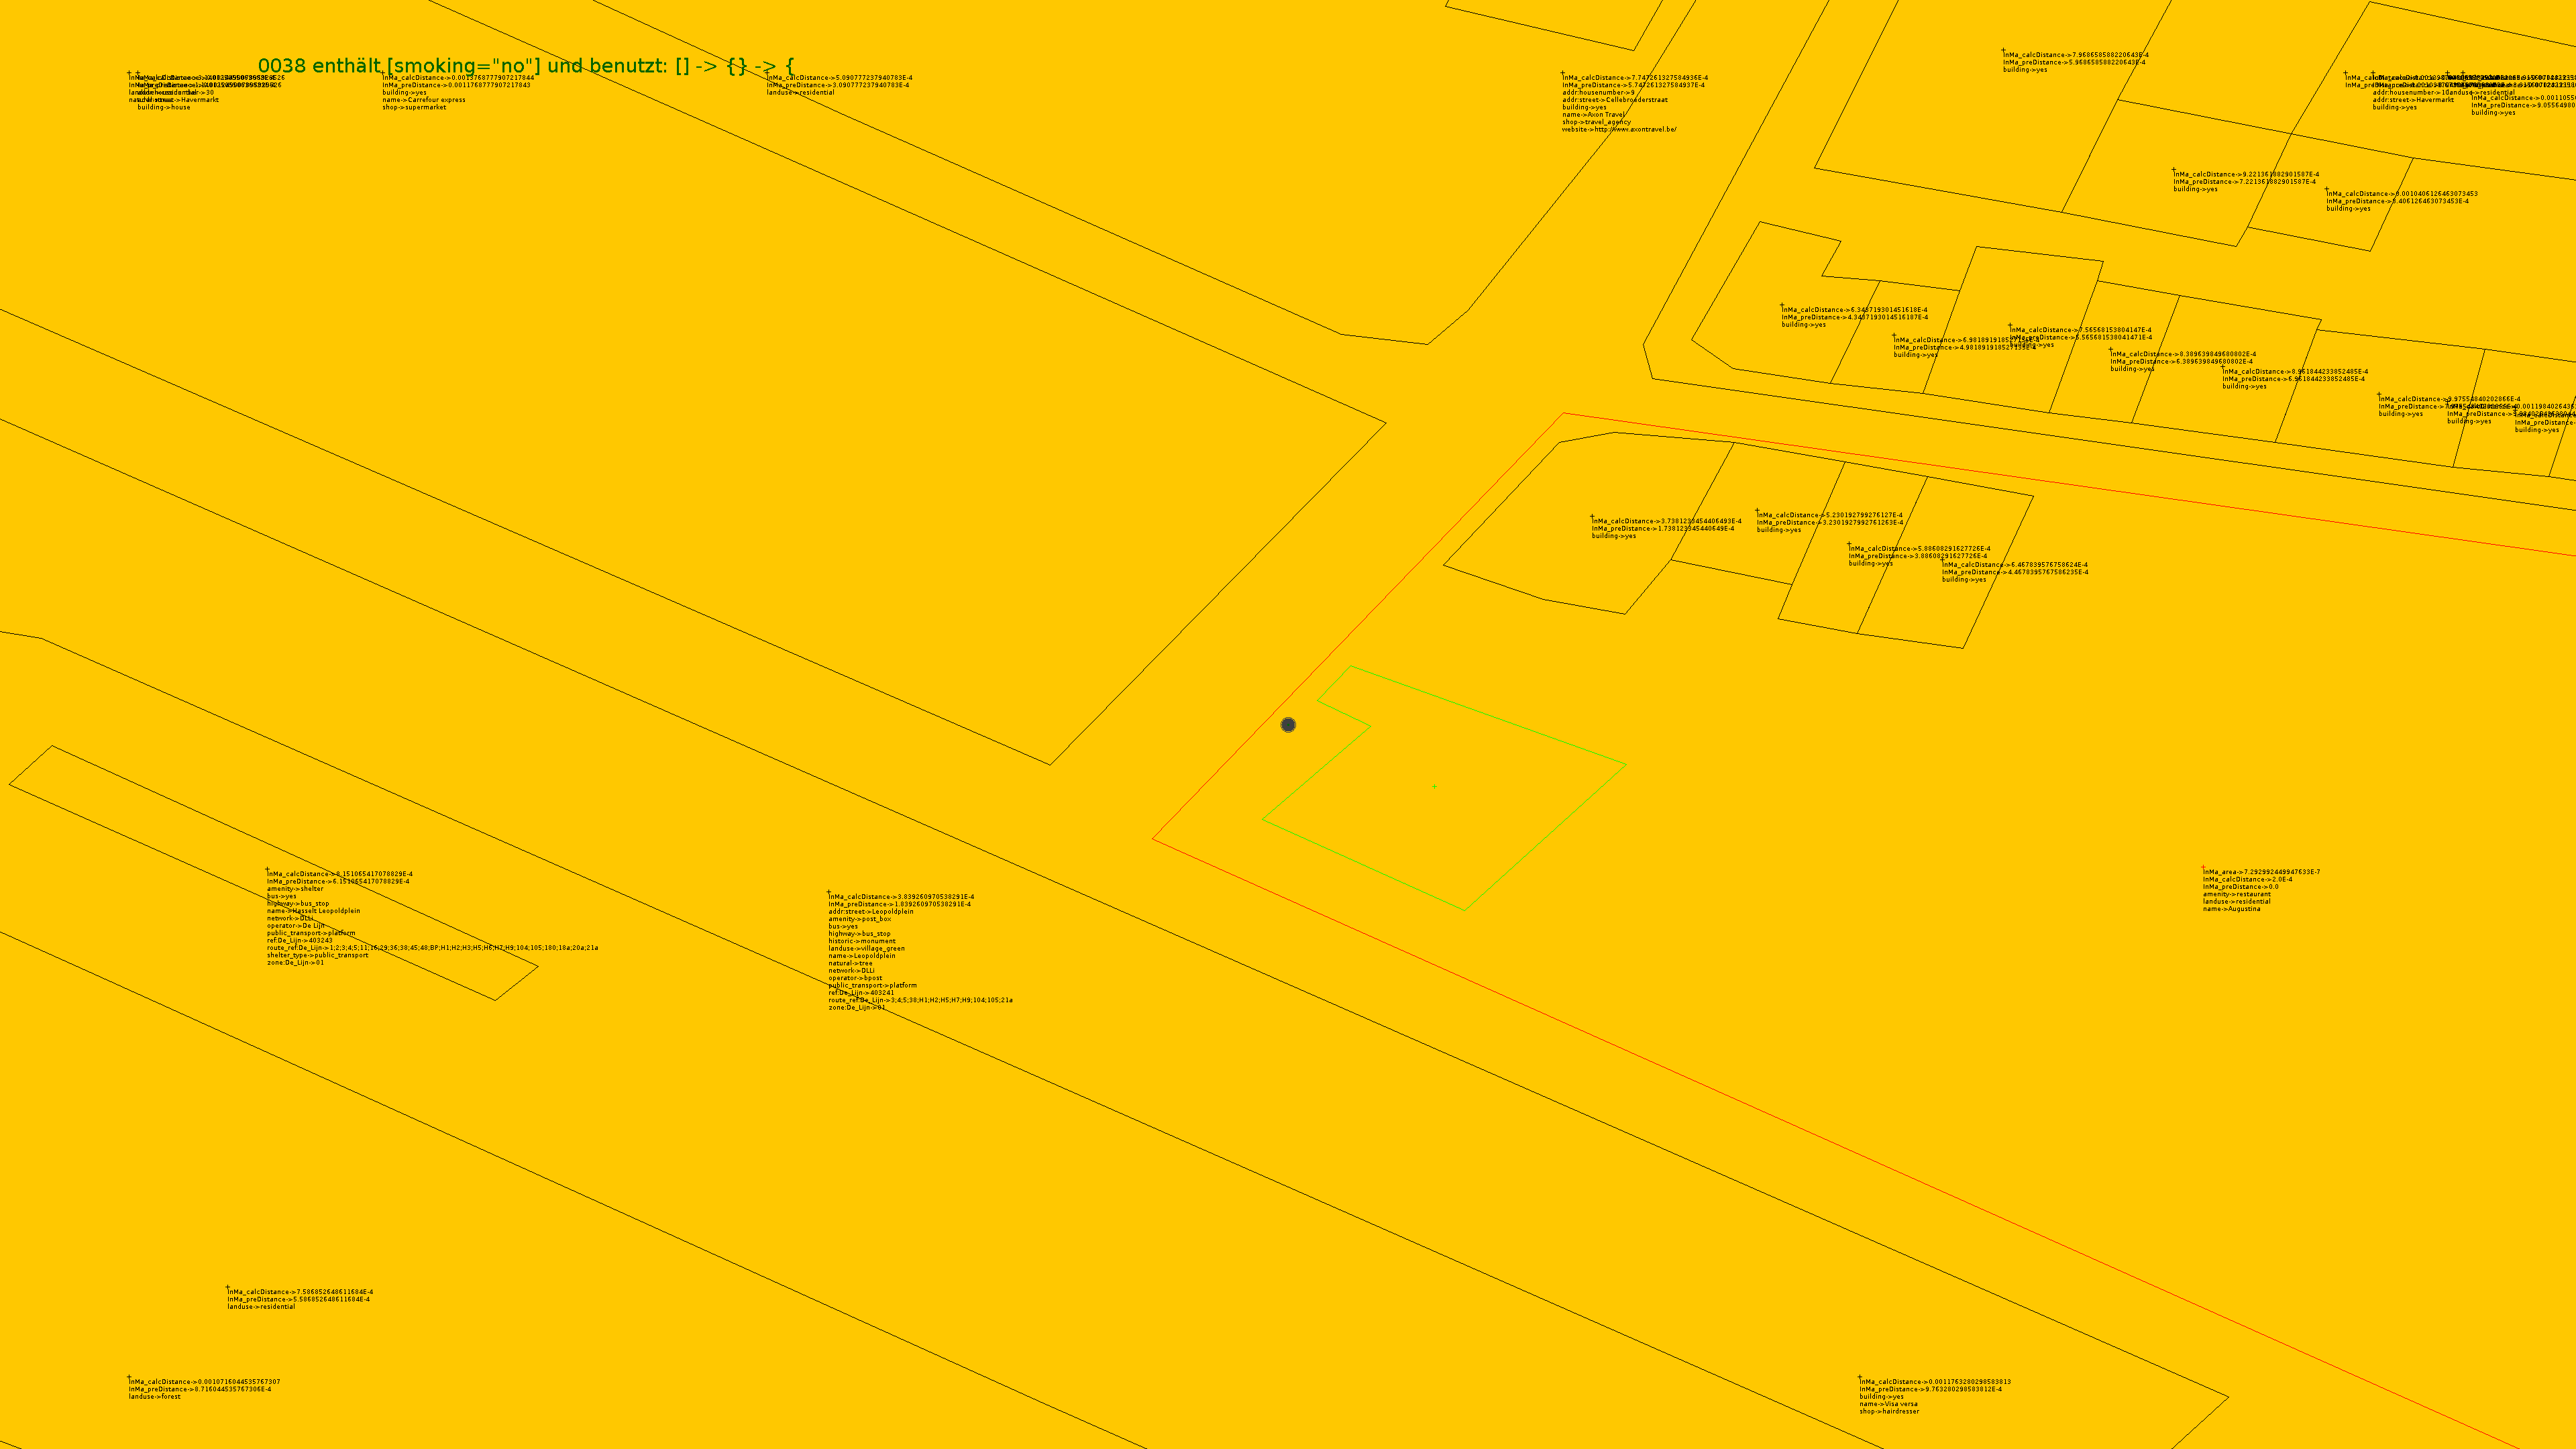
\includegraphics[width=\textwidth]{unvoll_naive}}
\end{frame}


\begin{frame}
  \frametitle{Umgebungspolygon}
  \Wider{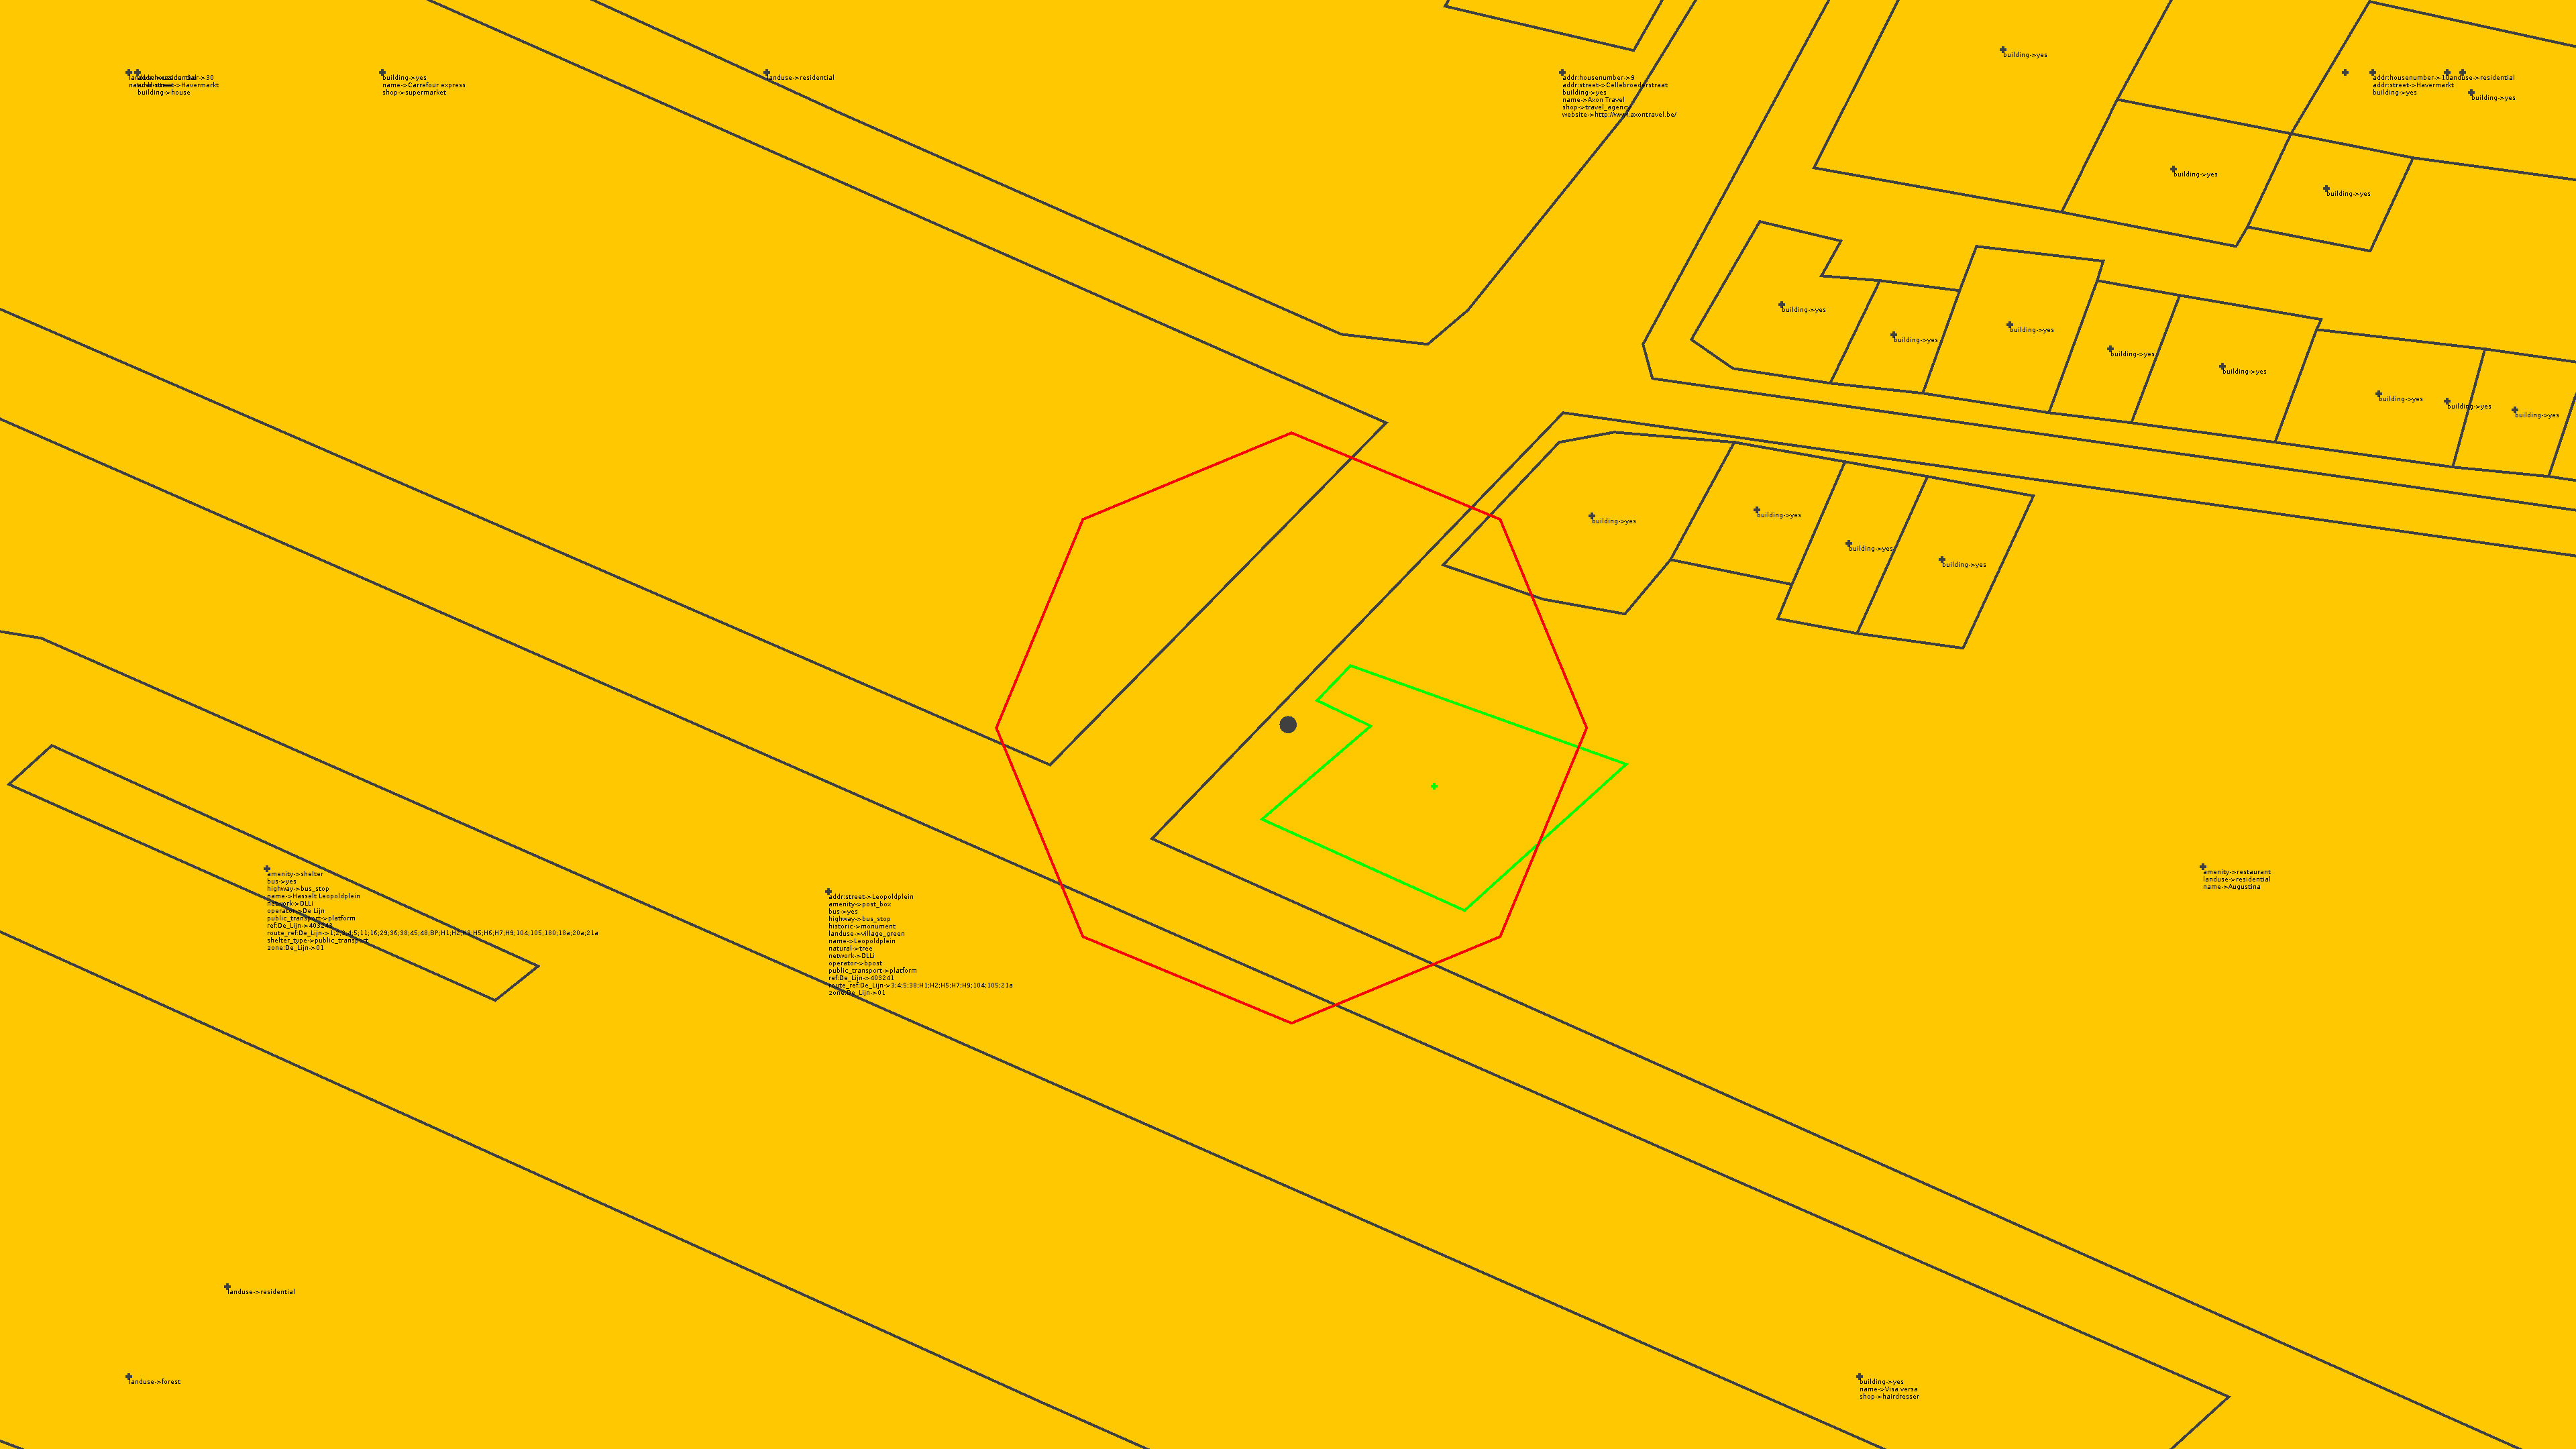
\includegraphics[width=\textwidth]{unvoll_full}}
\end{frame}


\begin{frame}
  \frametitle{Unvollständige Datensätze \hfill Nr. 38}
  \Wider{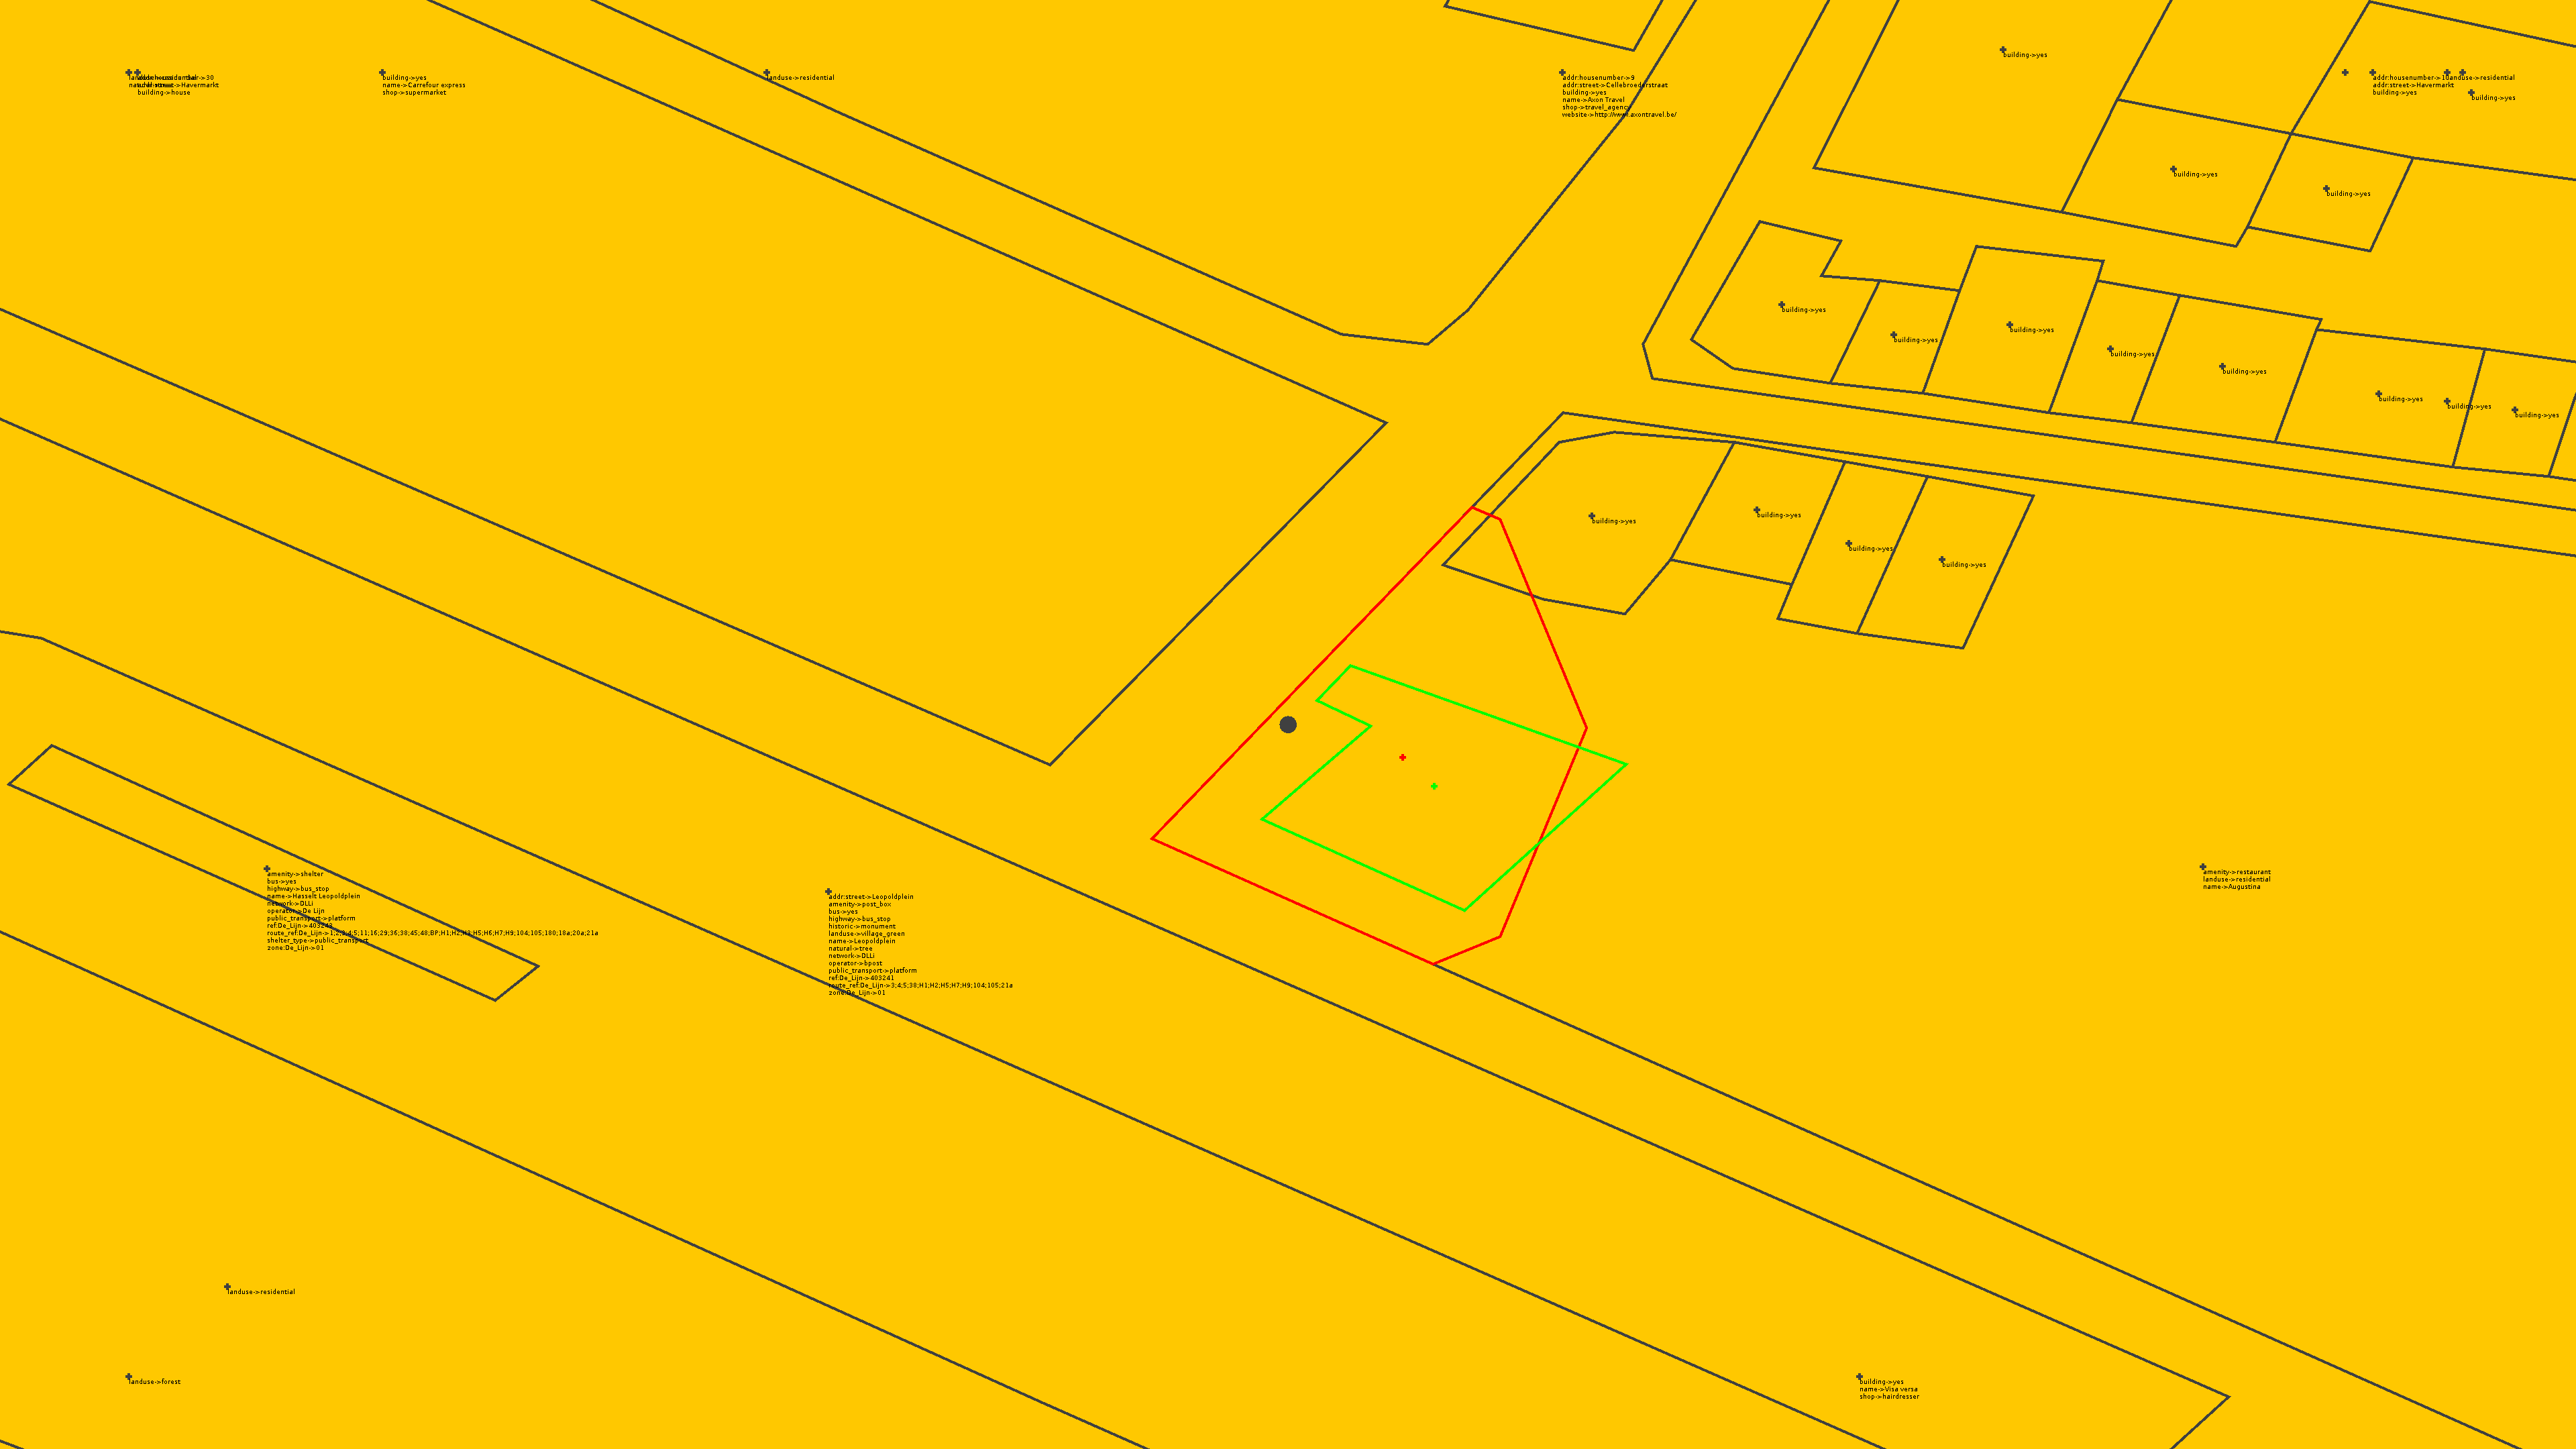
\includegraphics[width=\textwidth]{unvoll_result}}
\end{frame}


\begin{frame}
  \frametitle{Vollständiger Ansatz}
  \begin{center}
  \huge{Coverage = 74,6 \%}
  \end{center}
  \begin{center}
  Vorheriger Coverage =  69,8 \%
  \end{center}
\end{frame}

\begin{frame}
  \frametitle{Sonstige Verbesserungen}
  \begin{itemize}
    \item Partielle Gebäude zu einem zusammen gefügt
    \item OSM-Daten zwischengespeichert
    \item GPS-Daten aus Bildern auslesen
    \item GPS-Direction betrachtet (unnütz)
    \item Polygone erben Tags ihrer enthaltenen Punkte
%%%%%%%%%%%%%%%%%%%%%%%%%%%%%%%%%%%%%%%%%%%%%%%%%%%%%%%%%%%%%%%%%%%%%%%%%%%%%%%%
% Weitere Verbesserungen die wir gemacht haben, aber nicht groß erklären wollen.
%%%%%%%%%%%%%%%%%%%%%%%%%%%%%%%%%%%%%%%%%%%%%%%%%%%%%%%%%%%%%%%%%%%%%%%%%%%%%%%%
    \item ...
  \end{itemize}
\end{frame}

\begin{frame}[fragile]
  \frametitle{rules.xml Format}
  \lstset{language=XML,basicstyle=\scriptsize}
  \lstinputlisting{Rules.xml}
\end{frame}
